\chapter{Neurological and Neurocognitive Dysfunction}
\label{ch:neurological}

Neurological abnormalities represent one of the most consistently documented features of ME/CFS and provide critical insight into the pathophysiology of this complex disorder. The landmark NIH deep phenotyping study by Walitt et al.\ (2024) provided unprecedented detail on central nervous system dysfunction, identifying specific brain regions, neurotransmitter abnormalities, and mechanisms underlying the characteristic fatigue and cognitive impairment of ME/CFS~\cite{walitt2024deep}.

\section{Central Nervous System Abnormalities}
\label{sec:cns}

\subsection{Brain Structure and Function}

\subsubsection{Structural Neuroimaging Findings}

Multiple neuroimaging studies have documented structural brain abnormalities in ME/CFS patients, though findings have varied across studies due to differences in patient populations, imaging protocols, and analytical methods.

\paragraph{White Matter Abnormalities}
Several studies have reported increased white matter hyperintensities (WMH) in ME/CFS patients compared to healthy controls. These hyperintensities, visible on T2-weighted and FLAIR MRI sequences, may indicate demyelination, axonal loss, or microvascular damage. The distribution of WMH in ME/CFS patients tends to involve:
\begin{itemize}
    \item Periventricular white matter
    \item Subcortical regions
    \item Frontal and temporal lobes
\end{itemize}

The clinical significance of these findings remains debated, as similar changes occur with normal aging and various medical conditions. However, the presence of WMH in younger ME/CFS patients suggests pathological processes beyond typical age-related changes.

\paragraph{Gray Matter Volume Changes}
Voxel-based morphometry (VBM) studies have revealed regional gray matter volume reductions in ME/CFS patients. Commonly affected regions include:
\begin{itemize}
    \item Prefrontal cortex --- associated with executive function and decision-making
    \item Anterior cingulate cortex --- involved in attention, emotion, and autonomic regulation
    \item Hippocampus --- critical for memory consolidation
    \item Basal ganglia --- implicated in motor control and reward processing
    \item Insula --- integrating interoceptive signals and emotional processing
\end{itemize}

The correlation between regional volume changes and specific symptom domains supports a neuroanatomical basis for the cognitive and autonomic dysfunction characteristic of ME/CFS.

\subsubsection{Functional Neuroimaging: The NIH Deep Phenotyping Study}
\label{sec:nih-fmri}

The 2024 NIH study by Walitt et al.\ employed functional MRI during motor tasks to identify specific brain regions with abnormal activation patterns in PI-ME/CFS patients~\cite{walitt2024deep}. This study, involving 17 PI-ME/CFS patients and 21 matched healthy controls, provided the most rigorous functional neuroimaging data to date.

\paragraph{Temporal-Parietal Junction Dysfunction}
A critical finding was abnormally reduced activity in the temporal-parietal junction (TPJ) during effort-based decision-making tasks. The TPJ is a heteromodal association cortex located at the intersection of the temporal and parietal lobes, integrating information from multiple sensory modalities and playing essential roles in:

\begin{itemize}
    \item \textbf{Agency and intention attribution} --- distinguishing self-generated from externally generated actions
    \item \textbf{Effort allocation decisions} --- evaluating the cost-benefit ratio of physical and cognitive exertion
    \item \textbf{Attentional reorienting} --- shifting focus in response to unexpected stimuli
    \item \textbf{Social cognition} --- theory of mind and perspective-taking
    \item \textbf{Bodily self-consciousness} --- integrating multisensory signals about body ownership
\end{itemize}

The reduced TPJ activity in ME/CFS patients suggests a fundamental disruption in the brain's ability to accurately estimate effort requirements and allocate resources appropriately. This finding provides a neuroanatomical substrate for the characteristic mismatch between perceived capability and actual performance that defines the ME/CFS experience.

\paragraph{Motor Cortex Hyperactivity}
Paradoxically, while the TPJ showed reduced activation, the motor cortex demonstrated sustained hyperactivity during fatiguing grip tasks in ME/CFS patients. Key observations included:

\begin{itemize}
    \item Motor cortex remained abnormally active despite declining grip force output
    \item No evidence of peripheral muscle fatigue on electromyography
    \item Dissociation between central motor drive and peripheral performance
    \item Inefficient neural recruitment patterns requiring excessive cortical activation for submaximal force production
\end{itemize}

This pattern indicates that fatigue in ME/CFS originates centrally rather than peripherally. The motor cortex continues to ``try harder'' even as actual force production declines, suggesting a breakdown in the feedback mechanisms that normally calibrate effort to output.

\paragraph{Effort Preference Alteration: A New Paradigm}
Perhaps the most conceptually important finding from the NIH study was the identification of altered effort preference as a defining feature of PI-ME/CFS, distinct from physical fatigue (muscle exhaustion) or central fatigue (reduced motor cortex output). Walitt et al.\ proposed that:

\begin{quote}
``Fatigue may arise from a mismatch between what someone thinks they can achieve and what their bodies perform.''
\end{quote}

This reconceptualization has profound implications for understanding ME/CFS:

\begin{enumerate}
    \item \textbf{Not malingering or deconditioning}: The brain genuinely perceives effort requirements inaccurately, leading to appropriate behavioral responses to faulty signals.

    \item \textbf{Integrative dysfunction}: The TPJ normally synthesizes multiple information streams (interoceptive, proprioceptive, motivational) to generate effort estimates. In ME/CFS, this integration fails.

    \item \textbf{Protective mechanism gone awry}: The brain may be responding to genuine danger signals (inflammation, metabolic dysfunction) but miscalibrating the protective response.

    \item \textbf{Treatment implications}: Interventions targeting effort perception and decision-making networks may be more effective than those addressing peripheral fatigue.
\end{enumerate}

\begin{hypothesis}[Maladaptive Sickness Behavior Program]
ME/CFS symptoms may represent an evolutionarily conserved ``sickness behavior'' program---normally protective during acute infection---that becomes chronically activated due to persistent immune signaling. The TPJ, which normally integrates inflammatory signals with effort allocation decisions, may misinterpret chronic low-grade inflammation as ongoing acute illness, inappropriately suppressing activity to ``conserve resources'' for an immune battle that has already concluded (or that persists at subclinical levels). This would explain why the fatigue feels so viscerally ``real'' and protective to patients: the brain is executing a legitimate survival program, but one triggered by faulty or persistent signals rather than current metabolic necessity.
\end{hypothesis}

\paragraph{Risk-Based Decision-Making Impairment}
During behavioral tasks requiring risk assessment and effort allocation, ME/CFS patients demonstrated:
\begin{itemize}
    \item Reduced selection of ``hard'' task options even when rewards were equivalent
    \item Difficulty sustaining effort on extended tasks
    \item Altered subjective perception of task difficulty
    \item Normal motivation levels despite reduced effort output
\end{itemize}

These findings indicate that the problem lies not in willingness to exert effort (motivation) but in the neural computation of what constitutes acceptable effort levels.

\subsubsection{PET Scan Metabolic Findings}

Positron emission tomography (PET) studies have revealed regional hypometabolism in ME/CFS patients, indicating reduced glucose utilization and neuronal activity. Commonly affected regions include:

\begin{itemize}
    \item Brainstem nuclei --- potentially explaining autonomic dysfunction
    \item Basal ganglia --- correlating with motor symptoms and fatigue
    \item Medial prefrontal cortex --- associated with executive dysfunction
    \item Posterior parietal cortex --- linked to attention and spatial processing deficits
\end{itemize}

The pattern of hypometabolism overlaps significantly with regions showing structural and functional abnormalities, supporting a coherent picture of multifocal brain dysfunction.

\subsubsection{SPECT Perfusion Abnormalities}

Single-photon emission computed tomography (SPECT) studies have documented reduced regional cerebral blood flow (rCBF) in ME/CFS patients. Characteristic findings include:

\begin{itemize}
    \item Global reduction in cortical perfusion (10--15\% below controls)
    \item Focal hypoperfusion in temporal, frontal, and parietal regions
    \item Correlation between perfusion deficits and cognitive symptom severity
    \item Exacerbation of perfusion abnormalities following physical or cognitive exertion
\end{itemize}

The persistence of perfusion deficits across multiple studies and imaging modalities strongly supports cerebrovascular dysfunction as a contributor to ME/CFS symptoms.

\subsection{Neurotransmitter Abnormalities}
\label{sec:neurotransmitters}

\subsubsection{Catecholamine Pathway Dysregulation: CSF Findings}

The NIH deep phenotyping study provided the first direct evidence linking cerebrospinal fluid (CSF) catecholamine abnormalities to ME/CFS symptoms~\cite{walitt2024deep}. This represents a major advance in understanding the neurochemical basis of the disease.

\paragraph{Reduced CSF Catecholamines}
Lumbar puncture analysis revealed significantly reduced concentrations of catecholamines and their metabolites in ME/CFS patients compared to healthy controls:

\begin{itemize}
    \item \textbf{Dopamine and metabolites}: Lower levels of homovanillic acid (HVA), the primary dopamine metabolite
    \item \textbf{Norepinephrine and metabolites}: Reduced concentrations affecting arousal, attention, and stress responses
    \item \textbf{DHPG (3,4-dihydroxyphenylglycol)}: Significantly reduced levels of this norepinephrine metabolite, indicating decreased central noradrenergic activity
    \item \textbf{Epinephrine}: Decreased levels impacting energy mobilization
\end{itemize}

The DHPG finding is particularly significant because DHPG is the primary intraneuronal metabolite of norepinephrine, produced when norepinephrine is broken down within noradrenergic neurons. Low CSF DHPG specifically indicates reduced norepinephrine turnover in the central nervous system, pointing to hypofunction of the locus coeruleus and other noradrenergic nuclei.

\paragraph{Clinical Correlations}
The study established direct correlations between CSF catecholamine levels and clinical measures:

\begin{itemize}
    \item \textbf{Motor performance}: Lower catecholamines correlated with reduced grip strength endurance and slower reaction times
    \item \textbf{Effort-related behaviors}: Catecholamine deficits predicted reduced selection of ``hard'' tasks in decision-making paradigms
    \item \textbf{Cognitive impairment}: Memory and executive function scores correlated with dopamine metabolite levels
    \item \textbf{Fatigue severity}: Subjective fatigue ratings inversely correlated with norepinephrine concentrations
\end{itemize}

This establishes, for the first time, a direct biochemical pathway linking specific neurotransmitter abnormalities to the core symptoms of ME/CFS.

% Insert Figure: Normal Catecholamine Synthesis
% Figure: Normal Catecholamine Synthesis
% Efficient production of norepinephrine and epinephrine from tyrosine

\begin{figure}[htbp]
\centering
\begin{tikzpicture}[scale=0.75, every node/.style={scale=0.75},
    % Styles
    process/.style={draw=green!70!black, fill=green!10, very thick, rounded corners, text width=4.5cm, align=center, minimum height=1.1cm},
    output/.style={draw=green!70!black, fill=green!25, very thick, rounded corners, text width=4.5cm, align=center, minimum height=1.1cm},
    arrow/.style={-latex, very thick, green!70!black},
    note/.style={font=\small\itshape, text width=3.5cm, align=center},
]

% Title
\node[font=\large\bfseries, green!70!black] at (0, 9.5) {Normal Catecholamine Synthesis};

% Tyrosine
\node[process] (tyrosine) at (0, 8) {\textbf{Tyrosine}\\(from dietary protein)};

% Step 1: Tyrosine hydroxylase
\node[process] (th) at (0, 6) {\textbf{Tyrosine Hydroxylase}\\+ BH\textsubscript{4}, Fe, O\textsubscript{2}};
\draw[arrow] (tyrosine) -- (th);
\node[note, right=0.8cm of th] {Rate-limiting step\\Requires ATP};

% L-DOPA
\node[process] (ldopa) at (0, 4) {\textbf{L-DOPA}};
\draw[arrow] (th) -- (ldopa);

% Step 2: DOPA decarboxylase
\node[process] (ddc) at (0, 2) {\textbf{DOPA Decarboxylase}\\+ Vitamin B\textsubscript{6}};
\draw[arrow] (ldopa) -- (ddc);

% Dopamine
\node[process] (dopamine) at (0, 0) {\textbf{Dopamine}};
\draw[arrow] (ddc) -- (dopamine);

% Step 3: Dopamine beta-hydroxylase
\node[process] (dbh) at (0, -2) {\textbf{Dopamine $\beta$-Hydroxylase}\\+ Vitamin C, Copper};
\draw[arrow] (dopamine) -- (dbh);

% Norepinephrine
\node[output] (ne) at (0, -4) {\textbf{Norepinephrine}\\Alertness, focus, stress response};
\draw[arrow] (dbh) -- (ne);

% Epinephrine (optional path)
\node[output] (epi) at (0, -6) {\textbf{Epinephrine}\\(in adrenal medulla)\\Fight-or-flight response};
\draw[arrow] (ne) -- (epi);

% Key cofactors summary
\node[draw=green!70!black, fill=green!5, rounded corners, text width=10cm, align=left, font=\small] at (0, -8.5) {
\textbf{Essential cofactors:} BH\textsubscript{4} (tetrahydrobiopterin), Iron, Vitamin B\textsubscript{6}, Vitamin C, Copper. Adequate ATP is required for the rate-limiting tyrosine hydroxylase step.
};

\end{tikzpicture}
\caption{Normal catecholamine synthesis pathway from tyrosine to norepinephrine and epinephrine.}
\label{fig:catecholamine-normal}
\end{figure}


% Insert Figure: ME/CFS Catecholamine Synthesis Failure
% Figure: Catecholamine Synthesis Failure in ME/CFS
% Multiple bottlenecks reduce norepinephrine/epinephrine production

\begin{figure}[htbp]
\centering
\begin{tikzpicture}[
    node distance=2.5cm,
    scale=0.85, every node/.style={scale=0.85},
    % Styles
    normal/.style={draw=green!70!black, fill=green!10, very thick, rounded corners, text width=3cm, align=center, minimum height=0.9cm},
    impaired/.style={draw=red!70!black, fill=red!10, very thick, rounded corners, text width=3cm, align=center, minimum height=0.9cm},
    pathological/.style={draw=red!50!black, fill=red!20, very thick, rounded corners, text width=2.8cm, align=center, minimum height=0.9cm},
    arrow/.style={-latex, very thick, green!70!black},
    impaired-arrow/.style={-latex, very thick, red!70!black},
    cascade-arrow/.style={-latex, thick, orange!80!black, dashed},
    note/.style={font=\scriptsize\itshape, text width=2.5cm, align=center},
]

% Title
\node[font=\large\bfseries, red!70!black] at (0, 9) {ME/CFS: Catecholamine Synthesis Failure};

% LEFT SIDE: Impaired pathway
\begin{scope}[xshift=-4cm]
    % Tyrosine (normal)
    \node[normal] (tyrosine) at (0, 7) {Tyrosine};

    % Bottleneck 1: TH impaired
    \node[impaired] (th) at (0, 5) {Tyrosine Hydroxylase\\{\color{red}\textbf{ATP-limited}}\\{\color{red}\textbf{BH\textsubscript{4} depleted}}};
    \draw[impaired-arrow] (tyrosine) -- (th);
    \node[note, left=0.2cm of th, text=red!70!black] {Bottleneck 1:\\Energy deficit};

    % L-DOPA (reduced)
    \node[impaired] (ldopa) at (0, 3) {L-DOPA\\{\color{red}reduced}};
    \draw[impaired-arrow] (th) -- (ldopa);

    % DDC (may be impaired)
    \node[impaired] (ddc) at (0, 1.2) {DOPA Decarboxylase\\{\color{red}B\textsubscript{6} deficiency?}};
    \draw[impaired-arrow] (ldopa) -- (ddc);

    % Dopamine (reduced)
    \node[impaired] (dopamine) at (0, -0.6) {Dopamine\\{\color{red}reduced}};
    \draw[impaired-arrow] (ddc) -- (dopamine);

    % Bottleneck 2: DBH impaired
    \node[impaired] (dbh) at (0, -2.4) {Dopamine $\beta$-Hydroxylase\\{\color{red}\textbf{Vitamin C depleted}}};
    \draw[impaired-arrow] (dopamine) -- (dbh);
    \node[note, left=0.2cm of dbh, text=red!70!black] {Bottleneck 2:\\Cofactor depletion};

    % Severely reduced outputs
    \node[impaired, fill=red!25] (ne) at (0, -4.4) {\textbf{Norepinephrine}\\{\color{red}SEVERELY LOW}};
    \draw[impaired-arrow] (dbh) -- (ne);

    \node[impaired, fill=red!25] (epi) at (0, -6.2) {\textbf{Epinephrine}\\{\color{red}SEVERELY LOW}};
    \draw[impaired-arrow] (ne) -- (epi);
\end{scope}

% RIGHT SIDE: System failures
\begin{scope}[xshift=4.5cm]
    % Central deficit
    \node[pathological, minimum width=3.5cm] (deficit) at (0, 3) {\textbf{CATECHOLAMINE}\\  \textbf{DEFICIT}};

    % Five consequences
    \node[pathological] (autonomic) at (-2, 0.5) {\textbf{Autonomic}\\POTS\\Orthostatic\\intolerance};

    \node[pathological] (cognitive) at (2, 0.5) {\textbf{Cognitive}\\Brain fog\\Attention\\Memory};

    \node[pathological] (stress) at (-2, -2.5) {\textbf{Stress}\\Can't cope\\Crashes\\HPA issues};

    \node[pathological] (energy) at (2, -2.5) {\textbf{Energy}\\Metabolic\\slowdown\\Temperature};

    \node[pathological] (motivation) at (0, -5) {\textbf{Motivation}\\Anhedonia\\Avolition\\Low drive};

    % Cascade arrows
    \draw[cascade-arrow] (deficit) -- (autonomic);
    \draw[cascade-arrow] (deficit) -- (cognitive);
    \draw[cascade-arrow] (deficit) -- (stress);
    \draw[cascade-arrow] (deficit) -- (energy);
    \draw[cascade-arrow] (deficit) -- (motivation);
\end{scope}

% Arrow connecting left to right
\draw[cascade-arrow, line width=2pt] (-1.5, -5) -- (1.5, 3);

% Key point box
\node[draw=red!70!black, fill=red!5, rounded corners, text width=11cm, align=left, font=\small] at (0, -8) {
\textbf{Two major bottlenecks:} (1) Tyrosine hydroxylase impaired by ATP deficit and BH\textsubscript{4} depletion; (2) Dopamine $\beta$-hydroxylase impaired by vitamin C depletion. Low catecholamines cause autonomic dysfunction, cognitive impairment, and stress intolerance.
};

\end{tikzpicture}
\caption{ME/CFS catecholamine synthesis failure and systemic consequences.}
\label{fig:catecholamine-mecfs}
\end{figure}


Figures~\ref{fig:catecholamine-normal} and~\ref{fig:catecholamine-mecfs} illustrate the catecholamine synthesis pathway and two major bottlenecks in ME/CFS: (1) tyrosine hydroxylase impairment due to ATP deficit and BH\textsubscript{4} depletion, and (2) dopamine $\beta$-hydroxylase impairment due to vitamin C depletion.

\paragraph{Mechanistic Implications}
Central catecholamine deficiency could explain multiple ME/CFS features:

\begin{enumerate}
    \item \textbf{Fatigue}: Dopamine and norepinephrine are essential for maintaining arousal, motivation, and sustained attention. Deficiency produces profound fatigue without peripheral cause.

    \item \textbf{Cognitive dysfunction}: The prefrontal cortex depends on optimal dopamine levels for working memory and executive function. Both excess and deficiency impair cognition.

    \item \textbf{Autonomic dysregulation}: Norepinephrine is the primary neurotransmitter of the sympathetic nervous system. Central norepinephrine deficiency could produce the autonomic abnormalities characteristic of ME/CFS.

    \item \textbf{Reward processing}: Dopamine mediates reward anticipation and motivation. Deficiency could explain the reduced effort allocation observed in behavioral tasks.

    \item \textbf{Post-exertional malaise}: Physical exertion depletes catecholamines; if baseline levels are already low, even modest activity could produce profound neurotransmitter deficits and symptom exacerbation.
\end{enumerate}

\subsubsection{Tryptophan Pathway Alterations}

Metabolomic profiling of CSF in the NIH study also revealed abnormalities in tryptophan metabolism~\cite{walitt2024deep}. Tryptophan is the precursor for both serotonin and the kynurenine pathway, making its metabolism relevant to mood, cognition, and immune function.

\paragraph{Kynurenine Pathway Dysregulation}
The kynurenine pathway metabolizes approximately 95\% of dietary tryptophan and produces metabolites with diverse neuroactive effects:

\begin{itemize}
    \item \textbf{Quinolinic acid}: An NMDA receptor agonist and excitotoxin; elevated levels may contribute to neuroinflammation and cognitive dysfunction
    \item \textbf{Kynurenic acid}: An NMDA receptor antagonist with neuroprotective properties; imbalance with quinolinic acid may disrupt glutamatergic neurotransmission
    \item \textbf{3-hydroxykynurenine}: Generates reactive oxygen species, potentially contributing to oxidative stress
\end{itemize}

Immune activation, particularly interferon-gamma, stimulates the kynurenine pathway, providing a link between the immune abnormalities and neurological symptoms observed in ME/CFS.

% Insert Figure: Normal Tryptophan Metabolism
% Figure: Normal Tryptophan Metabolism
% Balanced split between serotonin and kynurenine pathways

\begin{figure}[htbp]
\centering
\begin{tikzpicture}[
    node distance=2.5cm and 4cm,  % Vertical and horizontal spacing
    % Styles
    process/.style={draw=green!70!black, fill=green!10, very thick, rounded corners, text width=3.8cm, align=center, minimum height=1cm},
    output/.style={draw=green!70!black, fill=green!25, very thick, rounded corners, text width=3.8cm, align=center, minimum height=1cm},
    arrow/.style={-latex, very thick, green!70!black},
    note/.style={font=\small\itshape, text width=3cm, align=center},
]

% Title
\node[font=\large\bfseries, green!70!black] (title) at (0, 0) {Normal Tryptophan Metabolism};

% Tryptophan input
\node[process, below=3cm of title] (trp) {\textbf{Tryptophan}\\(from dietary protein)};

% LEFT BRANCH: Serotonin pathway (5%)
\node[process, below left=2.5cm and 4.5cm of trp] (tph) {\textbf{TPH} (5\%)\\+ BH\textsubscript{4}, Fe, O\textsubscript{2}};
\draw[arrow] (trp) -- node[above left, font=\small] {5\%} (tph);

\node[process, below=of tph] (fivehttp) {\textbf{5-HTP}};
\draw[arrow] (tph) -- (fivehttp);

\node[output, below=of fivehttp] (serotonin) {\textbf{Serotonin (5-HT)}\\Mood, sleep\\Pain modulation};
\draw[arrow] (fivehttp) -- (serotonin);

% RIGHT BRANCH: Kynurenine pathway (95%)
\node[process, below right=2.5cm and 4.5cm of trp] (tdo) {\textbf{TDO/IDO} (95\%)\\Liver/immune cells};
\draw[arrow] (trp) -- node[above right, font=\small] {95\%} (tdo);

\node[process, below=of tdo] (kyn) {\textbf{Kynurenine}\\(KYN)};
\draw[arrow] (tdo) -- (kyn);

% Kynurenine splits
\node[output, below left=2.5cm and 2cm of kyn] (kyna) {\textbf{Kynurenic Acid}\\(KYNA)\\Neuroprotective};
\draw[arrow] (kyn) -- (kyna);

\node[output, below right=2.5cm and 2cm of kyn] (quin) {\textbf{Quinolinic Acid}\\(low levels)\\$\rightarrow$ NAD\textsuperscript{+}};
\draw[arrow] (kyn) -- (quin);

% Notes
\node[note, below=1.5cm of serotonin] {Small pathway\\essential for\\mood regulation};
\node[note, below=1.5cm of kyn] {Main pathway\\for NAD\textsuperscript{+}\\synthesis};

% Key point box
\node[draw=green!70!black, fill=green!5, rounded corners, text width=11cm, align=left, font=\small, below=8cm of kyn] {
\textbf{Normal balance:} 95\% of tryptophan goes to kynurenine pathway for NAD\textsuperscript{+} synthesis; 5\% to serotonin. Kynurenic acid (KYNA) is neuroprotective (NMDA antagonist). Quinolinic acid (QUIN) is kept at low, controlled levels.
};

\end{tikzpicture}
\caption{Normal tryptophan metabolism with balanced serotonin and kynurenine pathways.}
\label{fig:tryptophan-normal}
\end{figure}


% Insert Figure: ME/CFS Tryptophan Dysregulation
% Figure: Tryptophan-Kynurenine Dysregulation in ME/CFS
% Inflammation drives tryptophan away from serotonin, toxic metabolites accumulate

\begin{figure}[htbp]
\centering
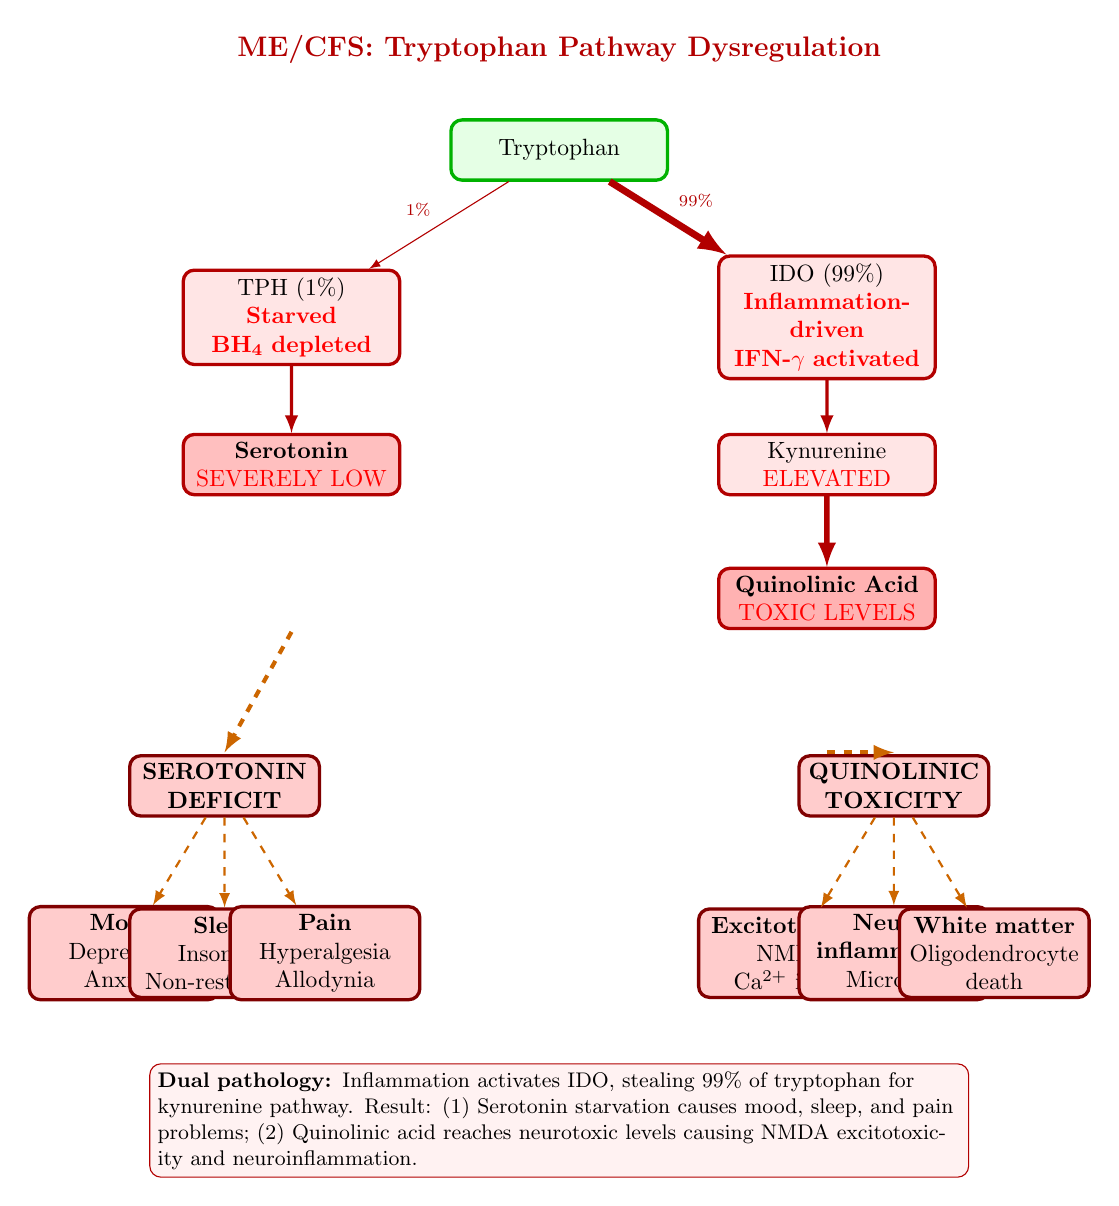
\begin{tikzpicture}[
    node distance=2.5cm,
    scale=0.85, every node/.style={scale=0.85},
    % Styles
    normal/.style={draw=green!70!black, fill=green!10, very thick, rounded corners, text width=3cm, align=center, minimum height=0.9cm},
    impaired/.style={draw=red!70!black, fill=red!10, very thick, rounded corners, text width=3cm, align=center, minimum height=0.9cm},
    pathological/.style={draw=red!50!black, fill=red!20, very thick, rounded corners, text width=2.6cm, align=center, minimum height=0.9cm},
    arrow/.style={-latex, very thick, green!70!black},
    impaired-arrow/.style={-latex, very thick, red!70!black},
    cascade-arrow/.style={-latex, thick, orange!80!black, dashed},
    note/.style={font=\scriptsize\itshape, text width=2.3cm, align=center},
]

% Title
\node[font=\large\bfseries, red!70!black] at (0, 9) {ME/CFS: Tryptophan Pathway Dysregulation};

% TOP: Dysregulated pathway
\begin{scope}[yshift=5cm]
    % Tryptophan
    \node[normal] (trp) at (0, 2.5) {Tryptophan};

    % LEFT: Serotonin - STARVED
    \node[impaired] (tph) at (-4, 0) {TPH (1\%)\\{\color{red}\textbf{Starved}}\\{\color{red}\textbf{BH\textsubscript{4} depleted}}};
    \draw[impaired-arrow, thin] (trp) -- node[above left, font=\scriptsize] {1\%} (tph);

    \node[impaired, fill=red!25] (serotonin) at (-4, -2.2) {\textbf{Serotonin}\\{\color{red}SEVERELY LOW}};
    \draw[impaired-arrow] (tph) -- (serotonin);

    % RIGHT: Kynurenine - HYPERACTIVE
    \node[impaired] (ido) at (4, 0) {IDO (99\%)\\{\color{red}\textbf{Inflammation-driven}}\\{\color{red}\textbf{IFN-$\gamma$ activated}}};
    \draw[impaired-arrow, line width=2.5pt] (trp) -- node[above right, font=\scriptsize] {99\%} (ido);

    \node[impaired] (kyn) at (4, -2.2) {Kynurenine\\{\color{red}ELEVATED}};
    \draw[impaired-arrow] (ido) -- (kyn);

    % Quinolinic acid - TOXIC
    \node[impaired, fill=red!30] (quin) at (4, -4.2) {\textbf{Quinolinic Acid}\\{\color{red}TOXIC LEVELS}};
    \draw[impaired-arrow, line width=2pt] (kyn) -- (quin);
\end{scope}

% BOTTOM: Dual pathology consequences
\begin{scope}[yshift=-4cm]
    % Serotonin deficit consequences (left)
    \node[pathological] (sero-def) at (-5, 2) {\textbf{SEROTONIN}\\  \textbf{DEFICIT}};

    \node[pathological] (mood) at (-6.5, -0.5) {\textbf{Mood}\\Depression\\Anxiety};
    \node[pathological] (sleep) at (-5, -0.5) {\textbf{Sleep}\\Insomnia\\Non-restorative};
    \node[pathological] (pain) at (-3.5, -0.5) {\textbf{Pain}\\Hyperalgesia\\Allodynia};

    \draw[cascade-arrow] (sero-def) -- (mood);
    \draw[cascade-arrow] (sero-def) -- (sleep);
    \draw[cascade-arrow] (sero-def) -- (pain);

    % Quinolinic acid consequences (right)
    \node[pathological] (quin-tox) at (5, 2) {\textbf{QUINOLINIC}\\  \textbf{TOXICITY}};

    \node[pathological] (excito) at (3.5, -0.5) {\textbf{Excitotoxicity}\\NMDA\\Ca\textsuperscript{2+} influx};
    \node[pathological] (neuroinf) at (5, -0.5) {\textbf{Neuro-}\\  \textbf{inflammation}\\Microglia};
    \node[pathological] (white) at (6.5, -0.5) {\textbf{White matter}\\Oligodendrocyte\\death};

    \draw[cascade-arrow] (quin-tox) -- (excito);
    \draw[cascade-arrow] (quin-tox) -- (neuroinf);
    \draw[cascade-arrow] (quin-tox) -- (white);
\end{scope}

% Arrows from pathway to consequences
\draw[cascade-arrow, line width=1.5pt] (-4, 0.3) -- (-5, -1.5);
\draw[cascade-arrow, line width=1.5pt] (4, -1.5) -- (5, -1.5);

% Key point box
\node[draw=red!70!black, fill=red!5, rounded corners, text width=12cm, align=left, font=\small] at (0, -7) {
\textbf{Dual pathology:} Inflammation activates IDO, stealing 99\% of tryptophan for kynurenine pathway. Result: (1) Serotonin starvation causes mood, sleep, and pain problems; (2) Quinolinic acid reaches neurotoxic levels causing NMDA excitotoxicity and neuroinflammation.
};

\end{tikzpicture}
\caption{ME/CFS tryptophan dysregulation causing serotonin deficit and quinolinic acid toxicity.}
\label{fig:tryptophan-mecfs}
\end{figure}


Figures~\ref{fig:tryptophan-normal} and~\ref{fig:tryptophan-mecfs} illustrate tryptophan metabolism dysregulation in ME/CFS. Inflammation-driven IDO overactivation diverts 99\% of tryptophan to the kynurenine pathway, starving serotonin synthesis while quinolinic acid reaches toxic levels.

\paragraph{Serotonin Synthesis}
Diversion of tryptophan into the kynurenine pathway reduces availability for serotonin synthesis. This may contribute to:
\begin{itemize}
    \item Sleep disturbances
    \item Mood symptoms
    \item Pain amplification
    \item Cognitive impairment
\end{itemize}

\subsubsection{Serotonergic Dysfunction}

Beyond tryptophan diversion, multiple lines of evidence suggest primary serotonergic abnormalities in ME/CFS:

\begin{itemize}
    \item Altered serotonin transporter binding on PET imaging
    \item Abnormal responses to serotonergic challenge tests
    \item Correlations between serotonin markers and fatigue severity
    \item Variable responses to serotonergic medications
\end{itemize}

The serotonergic system's role in regulating sleep, mood, pain perception, and autonomic function makes it a plausible contributor to the multisystem dysfunction of ME/CFS.

\subsubsection{Dopaminergic Dysfunction}

Dopamine abnormalities extend beyond the CSF findings to include:

\begin{itemize}
    \item Reduced dopamine transporter availability in basal ganglia
    \item Altered reward processing on functional imaging
    \item Blunted dopamine release in response to rewards
    \item Correlation between dopamine markers and motivational symptoms
\end{itemize}

The overlap between ME/CFS fatigue and the fatigue observed in Parkinson's disease and other dopaminergic disorders supports a common underlying mechanism.

\subsubsection{Norepinephrine and the Locus Coeruleus}

The locus coeruleus (LC), the primary source of brain norepinephrine, plays critical roles in:

\begin{itemize}
    \item Arousal and sleep-wake regulation
    \item Attention and cognitive flexibility
    \item Stress responses
    \item Autonomic nervous system modulation
\end{itemize}

LC dysfunction could explain the constellation of arousal, attention, and autonomic abnormalities in ME/CFS. Potential mechanisms include:

\begin{itemize}
    \item Neuroinflammation affecting LC neurons
    \item Autoantibodies targeting adrenergic receptors
    \item Metabolic stress impairing catecholamine synthesis
    \item Chronic stress-induced LC dysregulation
\end{itemize}

\subsubsection{GABAergic and Glutamatergic Imbalance}

Magnetic resonance spectroscopy (MRS) studies have revealed abnormalities in the balance between inhibitory (GABA) and excitatory (glutamate) neurotransmission in ME/CFS:

\begin{itemize}
    \item Elevated glutamate/glutamine in some brain regions
    \item Reduced GABA concentrations in others
    \item Altered glutamate/GABA ratios correlating with symptom severity
    \item Regional variations in neurochemical abnormalities
\end{itemize}

This excitatory/inhibitory imbalance could contribute to:
\begin{itemize}
    \item Sensory hypersensitivity
    \item Cognitive dysfunction
    \item Sleep disturbances
    \item Seizure susceptibility in some patients
\end{itemize}

\subsubsection{Cholinergic Dysfunction}

Acetylcholine abnormalities in ME/CFS have received less attention but may contribute to:

\begin{itemize}
    \item Cognitive impairment, particularly memory
    \item Autonomic dysfunction (parasympathetic arm)
    \item Sleep architecture abnormalities
    \item Muscle function
\end{itemize}

Autoantibodies against muscarinic acetylcholine receptors have been identified in some ME/CFS patients, providing a potential autoimmune mechanism for cholinergic dysfunction.

\subsection{Glial Cell Dysfunction}
\label{sec:glial}

\subsubsection{Microglial Activation and Neuroinflammation}

Microglia, the resident immune cells of the central nervous system, have emerged as key players in ME/CFS neuroinflammation. Evidence for microglial activation includes:

\begin{itemize}
    \item Elevated markers of microglial activation in CSF (soluble CD14, chitotriosidase)
    \item PET imaging showing increased translocator protein (TSPO) binding in specific brain regions
    \item Correlation between neuroinflammatory markers and symptom severity
    \item Persistence of microglial activation years after initial infection
\end{itemize}

Chronic microglial activation can produce:
\begin{itemize}
    \item Sustained release of pro-inflammatory cytokines (IL-1$\beta$, TNF-$\alpha$, IL-6)
    \item Oxidative stress through reactive oxygen species production
    \item Glutamate release contributing to excitotoxicity
    \item Disruption of synaptic pruning and plasticity
    \item Blood-brain barrier dysfunction
\end{itemize}

\subsubsection{Astrocyte Abnormalities}

Astrocytes perform essential functions including:
\begin{itemize}
    \item Neurotransmitter uptake and recycling
    \item Blood-brain barrier maintenance
    \item Metabolic support for neurons
    \item Synaptic modulation
    \item Ion homeostasis
\end{itemize}

Astrocyte dysfunction in ME/CFS may contribute to:
\begin{itemize}
    \item Impaired glutamate clearance and excitotoxicity
    \item Reduced metabolic support for neurons
    \item Blood-brain barrier compromise
    \item Abnormal synaptic transmission
\end{itemize}

Elevated GFAP (glial fibrillary acidic protein) in some ME/CFS patients suggests astrocyte reactivity, though findings have been inconsistent.

\subsubsection{Oligodendrocyte Function}

Oligodendrocytes produce the myelin sheaths essential for rapid nerve conduction. Potential abnormalities include:

\begin{itemize}
    \item Demyelination contributing to white matter hyperintensities
    \item Impaired remyelination capacity
    \item Oxidative damage to oligodendrocytes
    \item Disrupted axon-glial signaling
\end{itemize}

The white matter changes observed on MRI in ME/CFS patients may reflect oligodendrocyte dysfunction, though the mechanisms remain to be fully elucidated.

\section{Autonomic Nervous System Dysfunction}
\label{sec:ans-pathophysiology}

Autonomic dysfunction is nearly universal in ME/CFS and contributes substantially to disability. The NIH deep phenotyping study provided quantitative documentation of specific autonomic abnormalities~\cite{walitt2024deep}.

\subsection{Sympathetic vs. Parasympathetic Imbalance}
\label{sec:autonomic-imbalance}

\subsubsection{Heart Rate Variability Studies}

Heart rate variability (HRV) provides a non-invasive window into autonomic function. The NIH study documented significantly diminished HRV in PI-ME/CFS patients compared to controls~\cite{walitt2024deep}, indicating:

\begin{itemize}
    \item \textbf{Reduced overall variability}: Lower standard deviation of NN intervals (SDNN), reflecting decreased overall autonomic modulation
    \item \textbf{Diminished high-frequency power}: Reduced HF-HRV, specifically reflecting decreased parasympathetic (vagal) activity
    \item \textbf{Altered low-frequency power}: Changes in LF-HRV, influenced by both sympathetic and parasympathetic activity
    \item \textbf{Abnormal LF/HF ratio}: Suggesting sympathovagal imbalance
\end{itemize}

\paragraph{Clinical Implications of Reduced HRV}
Diminished HRV in ME/CFS correlates with:
\begin{itemize}
    \item Greater fatigue severity
    \item Worse orthostatic intolerance
    \item Impaired cognitive function
    \item Reduced exercise capacity
    \item Poorer quality of life
\end{itemize}

Low HRV is also an independent predictor of cardiovascular morbidity and mortality in other populations, raising concerns about long-term cardiovascular outcomes in ME/CFS.

\subsubsection{Baroreflex Sensitivity}

The baroreflex maintains blood pressure stability through rapid adjustments in heart rate and vascular tone. The NIH study found diminished baroreflex cardiovagal gain in ME/CFS patients~\cite{walitt2024deep}, indicating:

\begin{itemize}
    \item Impaired ability to modulate heart rate in response to blood pressure changes
    \item Reduced parasympathetic responsiveness
    \item Delayed cardiovascular adaptation to postural changes
    \item Vulnerability to orthostatic stress
\end{itemize}

\paragraph{Baroreflex Testing Methods}
Several methods assess baroreflex function:
\begin{itemize}
    \item \textbf{Spontaneous baroreflex analysis}: Calculating the relationship between spontaneous blood pressure and R-R interval fluctuations
    \item \textbf{Valsalva maneuver}: Assessing heart rate and blood pressure responses to standardized straining
    \item \textbf{Neck suction/pressure}: Directly stimulating carotid baroreceptors
    \item \textbf{Pharmacological methods}: Using vasoactive drugs to manipulate blood pressure
\end{itemize}

\subsubsection{Evidence for Decreased Parasympathetic Activity}

Multiple lines of evidence converge on parasympathetic (vagal) dysfunction as a central feature of ME/CFS autonomic abnormalities:

\begin{enumerate}
    \item \textbf{Reduced HRV high-frequency power}: Direct measure of cardiac vagal modulation
    \item \textbf{Diminished baroreflex sensitivity}: Primarily mediated by vagal mechanisms
    \item \textbf{Pupillary abnormalities}: Altered pupil responses to light (parasympathetically mediated)
    \item \textbf{Gastrointestinal dysmotility}: Vagal nerve regulates gut function
    \item \textbf{Reduced respiratory sinus arrhythmia}: Vagally mediated heart rate variation with breathing
\end{enumerate}

The NIH study explicitly concluded that the autonomic findings indicated ``decreased parasympathetic activity''~\cite{walitt2024deep}, providing a unifying explanation for many ME/CFS symptoms.

\subsubsection{Sympathetic Nervous System Abnormalities}

While parasympathetic dysfunction is prominent, sympathetic abnormalities also occur:

\begin{itemize}
    \item \textbf{Resting sympathetic overactivity}: Elevated norepinephrine spillover, increased muscle sympathetic nerve activity
    \item \textbf{Impaired sympathetic reactivity}: Blunted responses to stressors despite elevated baseline
    \item \textbf{Regional sympathetic dysfunction}: Variable activation across different vascular beds
    \item \textbf{Catecholamine dysregulation}: Abnormal synthesis, release, and clearance
\end{itemize}

The combination of elevated baseline sympathetic activity with reduced reactivity creates a rigid, poorly adaptive autonomic system unable to respond appropriately to physiological challenges.

\subsection{Mechanisms of Orthostatic Intolerance}
\label{sec:orthostatic-mechanisms}

Orthostatic intolerance (OI) affects an estimated 70--90\% of ME/CFS patients and manifests as:
\begin{itemize}
    \item Postural orthostatic tachycardia syndrome (POTS)
    \item Neurally mediated hypotension (NMH)
    \item Orthostatic hypotension (OH)
    \item Combinations of the above
\end{itemize}

Dysautonomia and POTS are components of the ``Septad'' framework of frequently co-occurring conditions in ME/CFS (Section~\ref{sec:septad}). Small fiber neuropathy, another Septad component, may underlie autonomic dysfunction in a subset of patients, emphasizing the need for comprehensive evaluation of these interrelated pathophysiologies.

\subsubsection{Blood Volume Abnormalities}

Reduced blood volume is well-documented in ME/CFS and contributes to orthostatic intolerance:

\begin{itemize}
    \item \textbf{Plasma volume deficit}: 10--20\% reduction compared to healthy individuals
    \item \textbf{Red cell mass reduction}: Variable findings across studies
    \item \textbf{Total blood volume decrease}: Compromising cardiovascular reserve
    \item \textbf{Mechanisms}: Possibly involving renin-angiotensin-aldosterone system dysfunction, reduced erythropoietin, or increased capillary permeability
\end{itemize}

Hypovolemia reduces cardiac preload, compromising stroke volume and cardiac output, particularly during orthostatic stress.

\subsubsection{Vascular Dysfunction}

Multiple vascular abnormalities contribute to orthostatic intolerance:

\begin{itemize}
    \item \textbf{Impaired venoconstriction}: Reduced ability to mobilize venous blood during standing
    \item \textbf{Excessive venous pooling}: Blood accumulates in dependent vessels
    \item \textbf{Arterial dysregulation}: Abnormal resistance vessel responses
    \item \textbf{Endothelial dysfunction}: Impaired nitric oxide bioavailability
\end{itemize}

\subsubsection{Adrenergic Receptor Dysfunction}

Abnormalities in adrenergic receptor function may explain some autonomic symptoms:

\begin{itemize}
    \item \textbf{Beta-adrenergic receptor autoantibodies}: Identified in subsets of ME/CFS patients; may either activate or block receptors
    \item \textbf{Alpha-adrenergic abnormalities}: Altered vasoconstrictor responses
    \item \textbf{Receptor desensitization}: Chronic catecholamine exposure may downregulate receptors
    \item \textbf{Post-receptor signaling defects}: Abnormalities in G-protein coupling or second messenger systems
\end{itemize}

\subsubsection{Renin-Angiotensin-Aldosterone System}

The RAAS regulates blood volume and pressure through:
\begin{itemize}
    \item Sodium and water retention
    \item Vasoconstriction
    \item Sympathetic activation
\end{itemize}

Abnormalities in ME/CFS may include:
\begin{itemize}
    \item Reduced aldosterone response to orthostatic stress
    \item Impaired renin secretion
    \item Altered angiotensin II sensitivity
    \item Inappropriate natriuresis
\end{itemize}

\section{Peripheral Nervous System}
\label{sec:peripheral-nervous}

\subsection{Small Fiber Neuropathy}
\label{sec:sfn}

Small fiber neuropathy (SFN) affects thinly myelinated A-delta fibers and unmyelinated C fibers, which mediate pain, temperature, and autonomic functions. SFN has emerged as a significant finding in ME/CFS.

\subsubsection{Skin Biopsy Findings}

Punch skin biopsies with intraepidermal nerve fiber density (IENFD) measurement represent the gold standard for SFN diagnosis:

\begin{itemize}
    \item \textbf{Reduced IENFD}: Multiple studies report decreased nerve fiber density in ME/CFS patients
    \item \textbf{Correlation with symptoms}: Lower IENFD correlates with pain severity and autonomic dysfunction
    \item \textbf{Distal predominance}: Typical length-dependent pattern with greater abnormalities in feet than thighs
    \item \textbf{Prevalence}: Estimates range from 30--60\% of ME/CFS patients meeting criteria for SFN
\end{itemize}

\subsubsection{Autonomic Testing}

Quantitative sudomotor axon reflex testing (QSART) and related methods assess small fiber autonomic function:

\begin{itemize}
    \item \textbf{Reduced sweat output}: Indicating sudomotor dysfunction
    \item \textbf{Abnormal sweat gland innervation}: On skin biopsy analysis
    \item \textbf{Correlation with orthostatic intolerance}: SFN may contribute to autonomic dysregulation
\end{itemize}

\subsubsection{Pain Mechanisms}

SFN may explain chronic pain in ME/CFS through:

\begin{itemize}
    \item \textbf{Neuropathic pain}: Burning, tingling, electric shock sensations
    \item \textbf{Allodynia}: Pain from normally non-painful stimuli
    \item \textbf{Hyperalgesia}: Exaggerated pain responses
    \item \textbf{Central sensitization}: Peripheral nerve damage may trigger central pain amplification
\end{itemize}

\subsubsection{Potential Causes of SFN in ME/CFS}

\begin{itemize}
    \item Autoimmune mechanisms (ganglioside antibodies, sodium channel antibodies)
    \item Metabolic dysfunction (mitochondrial, oxidative stress)
    \item Chronic inflammation
    \item Microvascular abnormalities affecting nerve blood supply
    \item Direct viral damage (in post-infectious cases)
\end{itemize}

\subsection{Nerve Conduction Studies}

\subsubsection{Electrophysiological Findings}

Standard nerve conduction studies (NCS) assess large myelinated fiber function and are typically normal in ME/CFS, consistent with selective small fiber involvement. However, some studies report:

\begin{itemize}
    \item Subtle prolongation of distal latencies
    \item Reduced compound muscle action potential amplitudes
    \item Abnormal F-wave parameters
    \item Changes suggesting subclinical demyelination
\end{itemize}

\subsubsection{Implications}

The contrast between abnormal small fiber findings and relatively preserved large fiber function suggests:

\begin{itemize}
    \item Selective vulnerability of small fibers to ME/CFS pathophysiology
    \item Potential autoimmune targeting of specific nerve fiber populations
    \item Metabolic or oxidative stress preferentially affecting unmyelinated fibers
    \item Different pathophysiology from typical diabetic or inflammatory neuropathies
\end{itemize}

\subsection{Treatment of Small Fiber Neuropathy}
\label{sec:sfn-treatment}

Management of SFN in ME/CFS requires addressing both symptomatic relief and underlying mechanisms. Treatment strategies must be adapted for ME/CFS-specific considerations including medication sensitivity and post-exertional malaise.

\subsubsection{First-Line Neuropathic Pain Medications}

\paragraph{Gabapentinoids.}
Gabapentin and pregabalin remain first-line treatments for neuropathic pain based on NeuPSIG guidelines~\cite{Finnerup2015neuropathic}. Dosing recommendations below derive from these guidelines and clinical experience; individual titration is essential:

\begin{itemize}
    \item \textbf{Gabapentin}: Start 100--300~mg at bedtime; titrate slowly to 900--3600~mg/day in divided doses
    \item \textbf{Pregabalin}: Start 25--75~mg at bedtime; titrate to 150--600~mg/day in divided doses
    \item \textbf{Mechanism}: Bind alpha-2-delta subunit of voltage-gated calcium channels, reducing excitatory neurotransmitter release
    \item \textbf{Benefits}: Also improve sleep quality and may reduce central sensitization
    \item \textbf{ME/CFS considerations}: Start at lower doses due to common medication sensitivity; sedation may help or hinder depending on individual sleep patterns
\end{itemize}

\paragraph{Serotonin-Norepinephrine Reuptake Inhibitors (SNRIs).}
Duloxetine has FDA approval for diabetic peripheral neuropathy~\cite{Finnerup2015neuropathic}:

\begin{itemize}
    \item \textbf{Duloxetine}: Start 20--30~mg daily; target 60~mg daily (range 30--120~mg)
    \item \textbf{Venlafaxine}: Alternative SNRI; 150--225~mg/day extended-release
    \item \textbf{Mechanism}: Enhance descending pain inhibition pathways via norepinephrine and serotonin
    \item \textbf{Additional benefits}: May help comorbid depression and fatigue in some patients
    \item \textbf{Cautions}: Discontinuation syndrome with abrupt cessation; may increase blood pressure
\end{itemize}

\paragraph{Tricyclic Antidepressants.}
Low-dose tricyclics provide analgesic effects independent of antidepressant action:

\begin{itemize}
    \item \textbf{Amitriptyline}: Start 10~mg at bedtime; titrate to 25--75~mg (lower than antidepressant doses)
    \item \textbf{Nortriptyline}: Less sedating alternative; 10--75~mg at bedtime
    \item \textbf{Mechanism}: Block norepinephrine reuptake, sodium channels, and NMDA receptors
    \item \textbf{Benefits}: Improve sleep architecture; long clinical experience
    \item \textbf{Cautions}: Anticholinergic effects (dry mouth, constipation, urinary retention); cardiac effects at higher doses; morning sedation
\end{itemize}

\subsubsection{Topical Treatments}

Topical agents provide targeted relief with minimal systemic effects---particularly valuable in medication-sensitive ME/CFS patients:

\paragraph{Lidocaine.}
\begin{itemize}
    \item \textbf{5\% lidocaine patches}: Apply to painful areas for up to 12 hours daily
    \item \textbf{Mechanism}: Blocks sodium channels in peripheral nerves, reducing ectopic firing
    \item \textbf{Advantages}: Minimal systemic absorption; can be cut to size; well-tolerated
    \item \textbf{Limitations}: Localized effect only; works best for focal pain
\end{itemize}

\paragraph{Capsaicin.}
\begin{itemize}
    \item \textbf{Low-concentration cream (0.025--0.075\%)}: Apply 3--4 times daily
    \item \textbf{High-concentration patch (8\%)}: Single application by healthcare provider; effects last 3 months
    \item \textbf{Mechanism}: Depletes substance P from peripheral nerve endings; defunctionalizes TRPV1-expressing nociceptors
    \item \textbf{Cautions}: Initial burning sensation (usually diminishes with regular use); avoid mucous membranes and eyes
\end{itemize}

\subsubsection{Treatment of Underlying Causes}

\paragraph{Autoimmune SFN.}
When SFN has an autoimmune etiology (suggested by anti-ganglioside or anti-sodium channel antibodies), immunomodulation may be beneficial~\cite{Oaklander2016autoimmuneSFN}:

\begin{itemize}
    \item \textbf{IVIG}: 0.4~g/kg/day for 5 days, then monthly maintenance; case series evidence (low certainty) suggests improvement in pain and autonomic symptoms in autoimmune SFN, though RCT data are lacking~\cite{Liu2020IVIG}
    \item \textbf{Corticosteroids}: Short courses for acute flares; long-term use limited by side effects
    \item \textbf{Other immunomodulators}: Rituximab, azathioprine, mycophenolate in refractory cases
    \item \textbf{ME/CFS relevance}: Given autoimmune hypotheses in ME/CFS, autoimmune SFN testing should be considered in patients with prominent neuropathic features
\end{itemize}

\paragraph{Metabolic and Nutritional Support.}
Several supplements may support nerve regeneration. Note that evidence derives primarily from diabetic neuropathy populations; efficacy in ME/CFS-associated SFN has not been specifically studied:

\begin{itemize}
    \item \textbf{Alpha-lipoic acid}: 600--1800~mg daily; demonstrated efficacy in diabetic neuropathy RCTs~\cite{Ziegler2006ALA}; antioxidant and mitochondrial cofactor
    \item \textbf{Acetyl-L-carnitine}: 1500--3000~mg daily; supports neuronal energy metabolism; RCT evidence in diabetic neuropathy showing improved pain and nerve regeneration~\cite{Sima2005ALCAR}
    \item \textbf{B vitamins}: B12 (methylcobalamin 1000--5000~mcg), B6 (avoid excess >100~mg/day, which can cause neuropathy), B1 (benfotiamine 300--600~mg)
    \item \textbf{Mechanism}: Support mitochondrial function, reduce oxidative stress, provide nerve membrane substrates
\end{itemize}

\begin{warning}[Vitamin B6 Toxicity]
While B6 deficiency can cause neuropathy, excess pyridoxine supplementation (typically >200~mg/day chronically) can paradoxically cause a sensory neuropathy. Patients should not exceed 100~mg/day without medical supervision, and B6 levels should be checked if neuropathy worsens with supplementation.
\end{warning}

\subsubsection{ME/CFS-Specific Considerations}

Treatment of SFN in ME/CFS requires adaptation for this population:

\begin{itemize}
    \item \textbf{Start low, go slow}: Begin at 25--50\% of typical starting doses due to medication sensitivity
    \item \textbf{Single changes}: Add or adjust one medication at a time to identify responses
    \item \textbf{Sedation balance}: Sedating medications (gabapentin, amitriptyline) may help sleep but worsen daytime fatigue
    \item \textbf{Autonomic effects}: Many neuropathic pain medications affect autonomic function; monitor orthostatic symptoms
    \item \textbf{PEM awareness}: Exercise-based therapies sometimes recommended for neuropathy are contraindicated in ME/CFS due to PEM risk
    \item \textbf{Topical preference}: Consider topical agents first given lower systemic burden
\end{itemize}

\subsubsection{Treatment Algorithm}

The following algorithm represents a proposed approach synthesized from NeuPSIG guidelines~\cite{Finnerup2015neuropathic} and clinical experience with ME/CFS patients. It is not a validated clinical guideline:

\begin{enumerate}
    \item \textbf{Diagnosis confirmation}: Skin biopsy for IENFD; autonomic testing; screen for treatable causes (diabetes, B12 deficiency, autoantibodies)
    \item \textbf{Address underlying causes}: Treat autoimmune SFN with immunomodulation; correct nutritional deficiencies
    \item \textbf{First-line symptomatic}: Topical lidocaine for focal pain; low-dose gabapentinoid or TCA at bedtime
    \item \textbf{Second-line}: Add SNRI if inadequate response; consider combination therapy (e.g., gabapentinoid + TCA)
    \item \textbf{Adjunctive support}: Alpha-lipoic acid, acetyl-L-carnitine for neuroprotection (extrapolated from diabetic neuropathy evidence)
    \item \textbf{Refractory cases}: Pain medicine referral; interventional options; IVIG trial if autoimmune markers present
\end{enumerate}

\begin{open_question}[SFN Reversibility in ME/CFS]
Can small fiber neuropathy in ME/CFS patients be reversed with appropriate treatment? Case reports suggest IENFD can normalize after treating underlying conditions (e.g., autoimmune SFN with IVIG, diabetic SFN with glucose control). If ME/CFS-associated SFN has an autoimmune or inflammatory basis, early immunomodulation might prevent permanent nerve damage. Longitudinal studies with serial skin biopsies in treated patients would clarify whether nerve regeneration is achievable.
\end{open_question}

\section{Blood-Brain Barrier Dysfunction}
\label{sec:bbb}

The blood-brain barrier (BBB) normally restricts entry of cells, pathogens, and molecules from the bloodstream into the brain parenchyma. BBB dysfunction may contribute to neuroinflammation and neurological symptoms in ME/CFS.

\subsection{Evidence for Permeability Changes}

\begin{itemize}
    \item \textbf{CSF/serum albumin ratio}: Elevated in some ME/CFS patients, indicating increased permeability
    \item \textbf{Neuroimaging markers}: Subtle gadolinium enhancement suggesting leakage
    \item \textbf{Peripheral inflammatory markers in CSF}: Cytokines and chemokines crossing the barrier
    \item \textbf{Autoantibodies in CNS}: Entry of pathogenic antibodies
\end{itemize}

\subsection{Consequences for Neuroinflammation}

BBB dysfunction permits:

\begin{itemize}
    \item \textbf{Peripheral immune cell infiltration}: T cells, monocytes entering brain tissue
    \item \textbf{Cytokine entry}: Peripheral inflammatory mediators reaching the CNS
    \item \textbf{Autoantibody access}: Receptor-targeting antibodies affecting neural function
    \item \textbf{Pathogen penetration}: Viral particles or antigens entering the brain
\end{itemize}

\subsection{Transport Dysfunction}

Beyond passive permeability, active transport systems at the BBB may be dysfunctional:

\begin{itemize}
    \item \textbf{Glucose transporters}: Potentially explaining cerebral hypometabolism
    \item \textbf{Amino acid transporters}: Affecting neurotransmitter precursor availability
    \item \textbf{Drug efflux pumps}: Altering CNS drug concentrations
    \item \textbf{Receptor-mediated transcytosis}: Impaired transport of essential molecules
\end{itemize}

\section{Cerebral Blood Flow Abnormalities}
\label{sec:cerebral-blood-flow}

Cerebral blood flow (CBF) abnormalities are among the most consistently documented findings in ME/CFS and likely contribute substantially to cognitive symptoms.

% Insert Figure: Normal Cerebral Blood Flow
% Figure: Normal Cerebral Blood Flow
% Adequate perfusion meets brain's high metabolic demands

\begin{figure}[htbp]
\centering
\begin{tikzpicture}[
    node distance=2.5cm,  % Global minimum vertical spacing
    % Styles
    process/.style={draw=green!70!black, fill=green!10, very thick, rounded corners, text width=4.5cm, align=center, minimum height=1.2cm},
    output/.style={draw=green!50!black, fill=green!30, ultra thick, rounded corners, text width=4.5cm, align=center, minimum height=1.3cm},
    arrow/.style={-latex, very thick, green!70!black, line width=1.2pt},
    note/.style={font=\small\itshape, text width=3.5cm, align=left, green!40!black},
]

% Title
\node[font=\large\bfseries, green!70!black] (title) at (0, 0) {Normal Cerebral Blood Flow};

% Cardiac output
\node[process, below=3cm of title] (cardiac) {\textbf{Cardiac Output}\\Normal stroke volume\\Adequate blood pressure};

% Cerebral autoregulation
\node[process, below=of cardiac] (autoreg) {\textbf{Cerebral Autoregulation}\\Maintains flow 50--150 mmHg\\Vasodilation/constriction};
\draw[arrow] (cardiac) -- (autoreg);
\node[note, right=1.5cm of autoreg] {Adjusts vessel\\diameter to\\maintain flow};

% Normal CBF
\node[output, below=of autoreg] (cbf) {\textbf{Cerebral Blood Flow}\\50--60 mL/100g/min\\Meets O\textsubscript{2}/glucose demand};
\draw[arrow] (autoreg) -- (cbf);
\node[note, right=1.5cm of cbf] {Brain uses\\20\% of cardiac\\output at rest};

% Brain function
\node[output, below=of cbf] (brain) {\textbf{Normal Brain Function}\\Cognition intact\\Energy metabolism stable\\Neurotransmission normal};
\draw[arrow] (cbf) -- (brain);

% Key point box
\node[draw=green!70!black, fill=green!5, rounded corners, text width=10cm, align=left, font=\small, below=2.5cm of brain] {
\textbf{Key points:} The brain requires constant, high blood flow due to its enormous metabolic demands. Autoregulation maintains stable perfusion across a wide range of blood pressures. Adequate O\textsubscript{2} and glucose delivery, plus CO\textsubscript{2}/lactate removal, enable normal cognitive function.
};

\end{tikzpicture}
\caption{Normal cerebral blood flow regulation meeting brain metabolic demands.}
\label{fig:cerebral-hypoperfusion-normal}
\end{figure}


% Insert Figure: ME/CFS Cerebral Hypoperfusion
% Figure: Cerebral Hypoperfusion in ME/CFS
% Reduced blood flow causes brain energy crisis

\begin{figure}[htbp]
\centering
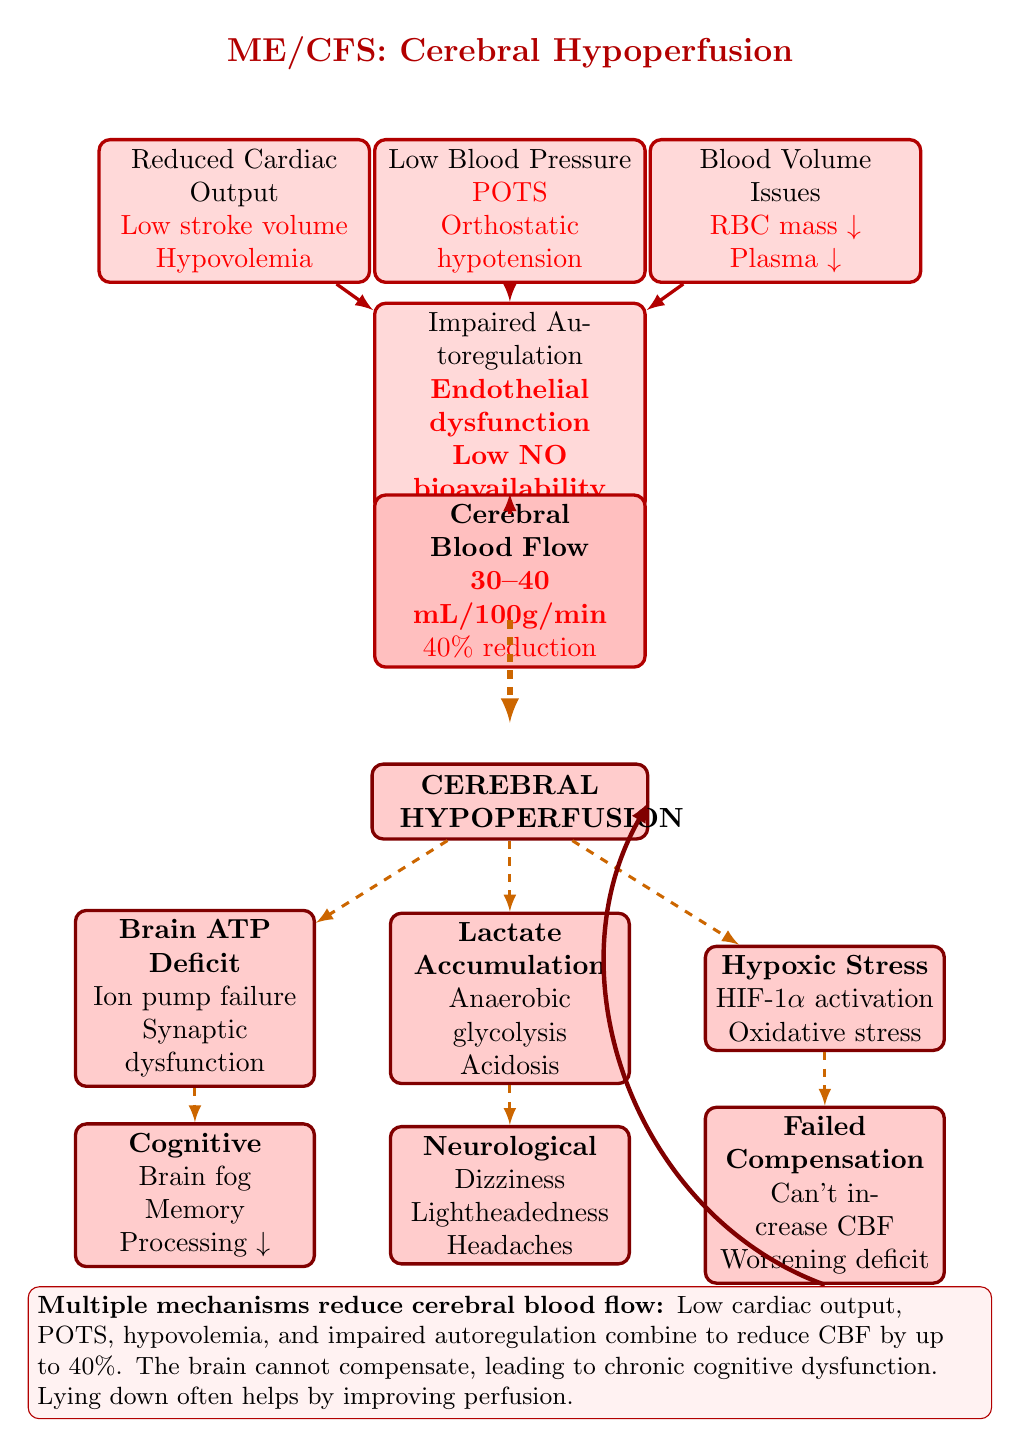
\begin{tikzpicture}[scale=1, every node/.style={scale=1},
    % Styles
    normal/.style={draw=green!70!black, fill=green!10, very thick, rounded corners, text width=3cm, align=center, minimum height=1cm},
    impaired/.style={draw=red!70!black, fill=red!15, very thick, rounded corners, text width=3.2cm, align=center, minimum height=1cm},
    severe/.style={draw=red!50!black, fill=red!25, ultra thick, rounded corners, text width=3.2cm, align=center, minimum height=1.1cm, drop shadow},
    pathological/.style={draw=red!50!black, fill=red!20, very thick, rounded corners, text width=2.8cm, align=center, minimum height=0.95cm},
    impaired-arrow/.style={-latex, very thick, red!70!black, line width=1.2pt},
    cascade-arrow/.style={-latex, thick, orange!80!black, dashed, line width=1.1pt},
    cycle-arrow/.style={-latex, ultra thick, red!50!black, line width=1.6pt},
    note/.style={font=\small\itshape, text width=2.4cm, align=left, red!60!black},
]

% Title
\node[font=\large\bfseries, red!70!black] at (0, 9) {ME/CFS: Cerebral Hypoperfusion};

% TOP: Impaired flow pathway
\begin{scope}[yshift=4.5cm]
    % Multiple contributors
    \node[impaired] (cardiac) at (-3.5, 2.5) {Reduced Cardiac\\Output\\{\color{red}Low stroke volume}\\{\color{red}Hypovolemia}};

    \node[impaired] (bp) at (0, 2.5) {Low Blood Pressure\\{\color{red}POTS}\\{\color{red}Orthostatic\\hypotension}};

    \node[impaired] (volume) at (3.5, 2.5) {Blood Volume\\Issues\\{\color{red}RBC mass $\downarrow$}\\{\color{red}Plasma $\downarrow$}};

    % Impaired autoregulation
    \node[impaired] (autoreg) at (0, 0) {Impaired Autoregulation\\{\color{red}\textbf{Endothelial dysfunction}}\\{\color{red}\textbf{Low NO bioavailability}}};
    \draw[impaired-arrow] (cardiac) -- (autoreg);
    \draw[impaired-arrow] (bp) -- (autoreg);
    \draw[impaired-arrow] (volume) -- (autoreg);

    % Reduced CBF
    \node[impaired, fill=red!25] (cbf) at (0, -2.2) {\textbf{Cerebral Blood Flow}\\{\color{red}\textbf{30--40 mL/100g/min}}\\{\color{red}40\% reduction}};
    \draw[impaired-arrow] (autoreg) -- (cbf);
\end{scope}

% BOTTOM: Cascade consequences
\begin{scope}[yshift=-3.5cm]
    % Central hypoperfusion
    \node[pathological, minimum width=3.5cm] (hypoperf) at (0, 3) {\textbf{CEREBRAL}\\  \textbf{HYPOPERFUSION}};

    % Three immediate consequences
    \node[pathological] (atp) at (-4, 0.5) {\textbf{Brain ATP}\\  \textbf{Deficit}\\Ion pump failure\\Synaptic dysfunction};

    \node[pathological] (lactate) at (0, 0.5) {\textbf{Lactate}\\  \textbf{Accumulation}\\Anaerobic glycolysis\\Acidosis};

    \node[pathological] (hypoxia) at (4, 0.5) {\textbf{Hypoxic Stress}\\HIF-1$\alpha$ activation\\Oxidative stress};

    \draw[cascade-arrow] (hypoperf) -- (atp);
    \draw[cascade-arrow] (hypoperf) -- (lactate);
    \draw[cascade-arrow] (hypoperf) -- (hypoxia);

    % Downstream symptoms
    \node[pathological] (cognitive) at (-4, -2) {\textbf{Cognitive}\\Brain fog\\Memory\\Processing $\downarrow$};

    \node[pathological] (neuro) at (0, -2) {\textbf{Neurological}\\Dizziness\\Lightheadedness\\Headaches};

    \node[pathological] (failed) at (4, -2) {\textbf{Failed}\\  \textbf{Compensation}\\Can't increase CBF\\Worsening deficit};

    \draw[cascade-arrow] (atp) -- (cognitive);
    \draw[cascade-arrow] (lactate) -- (neuro);
    \draw[cascade-arrow] (hypoxia) -- (failed);

    % Feedback loop
    \draw[cycle-arrow, bend left=50] (failed.south) to (hypoperf.east);
\end{scope}

% Arrow connecting top to bottom
\draw[cascade-arrow, line width=2pt] (0, 1.8) -- (0, 0.5);

% Key point box
\node[draw=red!70!black, fill=red!5, rounded corners, text width=12cm, align=left, font=\small] at (0, -7.5) {
\textbf{Multiple mechanisms reduce cerebral blood flow:} Low cardiac output, POTS, hypovolemia, and impaired autoregulation combine to reduce CBF by up to 40\%. The brain cannot compensate, leading to chronic cognitive dysfunction. Lying down often helps by improving perfusion.
};

\end{tikzpicture}
\caption{ME/CFS cerebral hypoperfusion cascade causing cognitive dysfunction.}
\label{fig:cerebral-hypoperfusion-mecfs}
\end{figure}


Figures~\ref{fig:cerebral-hypoperfusion-normal} and~\ref{fig:cerebral-hypoperfusion-mecfs} illustrate how multiple mechanisms reduce cerebral blood flow in ME/CFS (30--40 mL/100g/min vs.\ normal 50--60 mL/100g/min, a 40\% reduction).

\subsection{Reduced Regional Blood Flow}

Multiple neuroimaging modalities have demonstrated CBF reductions:

\begin{itemize}
    \item \textbf{Global hypoperfusion}: 10--20\% reduction in total cerebral blood flow
    \item \textbf{Regional deficits}: Particularly in frontal, temporal, and parietal regions
    \item \textbf{Brainstem hypoperfusion}: Potentially explaining autonomic dysfunction
    \item \textbf{Subcortical abnormalities}: Basal ganglia and thalamic hypoperfusion
\end{itemize}

\subsection{Correlation with Cognitive Symptoms}

CBF reductions correlate with specific cognitive deficits:

\begin{itemize}
    \item Frontal hypoperfusion → executive dysfunction, working memory impairment
    \item Temporal hypoperfusion → verbal memory deficits, language processing difficulties
    \item Parietal hypoperfusion → attention deficits, spatial processing impairment
    \item Global hypoperfusion → processing speed reduction, mental fatigue
\end{itemize}

\subsection{Mechanisms of Cerebral Hypoperfusion}

\begin{itemize}
    \item \textbf{Reduced cardiac output}: Secondary to autonomic dysfunction and blood volume deficits
    \item \textbf{Impaired cerebral autoregulation}: Inability to maintain CBF across blood pressure changes
    \item \textbf{Endothelial dysfunction}: Reduced nitric oxide-mediated vasodilation
    \item \textbf{Increased cerebrovascular resistance}: Vasoconstriction or structural changes
    \item \textbf{Neurovascular uncoupling}: Failure of blood flow to match metabolic demand
\end{itemize}

\subsection{Exacerbation with Exertion}

Importantly, cerebral perfusion abnormalities worsen following physical or cognitive exertion:

\begin{itemize}
    \item Further CBF reductions post-exercise
    \item Prolonged recovery of normal perfusion
    \item Correlation with post-exertional malaise severity
    \item Potential contribution to cognitive ``crashes'' following activity
\end{itemize}

\section{Auditory Processing Dysfunction and Tinnitus}
\label{sec:auditory-dysfunction}

Auditory symptoms represent an underrecognized but significant neurological manifestation of ME/CFS, with convergent evidence from functional, epidemiological, systematic, and anatomical studies establishing auditory dysfunction as a documented feature of the disease.

\subsection{Prevalence and Epidemiology}

\begin{achievement}[Tinnitus-ME/CFS Epidemiological Association]
\label{ach:schubert2021-tinnitus}
Schubert et al.~\cite{Schubert2021} provided the first large-scale epidemiological evidence linking ME/CFS to tinnitus in a population-based cohort of 124,609 individuals from the Dutch Lifelines study. ME/CFS patients demonstrated 1.57 times higher odds (OR 1.568, p<0.05) of experiencing constant tinnitus compared to healthy controls, identifying ME/CFS as a novel disease associate for tinnitus beyond traditional audiological causes such as noise exposure, age-related hearing loss, and cardiovascular disease.
\end{achievement}

This finding aligns with earlier cohort studies and patient surveys reporting tinnitus prevalence ranging from 48\% to 78\% in ME/CFS patients, substantially higher than the 10--15\% prevalence in the general population.

\begin{achievement}[Systematic Evidence for Auditory Dysfunction]
\label{ach:skare2024-ear}
A 2024 systematic review by Skare et al.~\cite{Skare2024} synthesized evidence from 172 articles (1990--2024) documenting ear abnormalities across ME/CFS, fibromyalgia, long-COVID syndrome, postural orthostatic tachycardia syndrome (PoTS), and related conditions. The review identified cochlear complaints---including tinnitus, hearing loss, and hyperacusis---as the most frequent auditory findings in ME/CFS. Four pathophysiological mechanisms were proposed: (1) viral effects on cochlear or central auditory structures, (2) vascular impairment reducing blood flow to the cochlea and brainstem, (3) autoimmune reactions targeting inner ear antigens, and (4) oxidative stress damaging cochlear hair cells and auditory neurons.
\end{achievement}

The systematic review recommended that all ME/CFS patients with audiological complaints receive ENT consultation and formal audiometry to assess the nature and severity of auditory dysfunction.

\subsection{Functional Auditory Processing Deficits}

Beyond subjective tinnitus complaints, objective evidence demonstrates specific auditory processing impairments in ME/CFS patients.

\begin{achievement}[Selective Auditory Processing Impairment]
\label{ach:johnson1996-auditory}
Johnson et al.~\cite{Johnson1996} demonstrated modality-specific cognitive impairment in a controlled comparison of 20 CFS patients, 20 multiple sclerosis (MS) patients, and 20 healthy controls. CFS patients showed differential impairment on auditory versus visual processing tasks, while MS patients showed equal impairment on both modalities. This pattern suggests specific dysfunction in central auditory pathways rather than general cognitive slowing, distinguishing the ME/CFS cognitive profile from the more global impairment observed in other neurological conditions.
\end{achievement}

Functional MRI studies have further documented that CFS patients utilize more extensive brain regions for auditory processing compared to controls, requiring greater neural recruitment and elevated source current to achieve equivalent performance. This suggests inefficient auditory processing requiring compensatory activation of additional neural networks.

\subsection{Neuroanatomical Substrate: Brainstem Dysfunction}

The functional auditory deficits and elevated tinnitus prevalence in ME/CFS are explained by documented structural and functional abnormalities in brainstem regions critical for auditory processing.

\begin{achievement}[Brainstem Structural Abnormalities]
\label{ach:nelson2021-brainstem}
Nelson et al.~\cite{Nelson2021} synthesized MRI evidence from 11 studies demonstrating structural and functional brainstem abnormalities in ME/CFS patients. The brainstem contains the primary central auditory pathway structures:

\begin{itemize}
    \item \textbf{Cochlear nucleus} (medulla) --- receives input from cochlear nerve; first central processing station
    \item \textbf{Superior olivary complex} (pons) --- sound localization via interaural time and intensity differences
    \item \textbf{Lateral lemniscus} --- ascending auditory pathway connecting lower and upper brainstem
    \item \textbf{Inferior colliculus} (midbrain) --- integration of ascending auditory information before thalamic relay
\end{itemize}

Dysfunction in these structures provides a neuroanatomical substrate explaining both the auditory processing deficits documented by Johnson et al.~\cite{Johnson1996} and the increased tinnitus prevalence observed by Schubert et al.~\cite{Schubert2021}.
\end{achievement}

Importantly, brainstem abnormalities in ME/CFS extend beyond auditory pathways to include autonomic control centers (see Section~\ref{sec:ans-pathophysiology}), arousal systems (locus coeruleus), and sensory integration regions. This explains the co-occurrence of auditory symptoms with autonomic dysfunction, sleep disturbances, and sensory hypersensitivity---all manifestations of brainstem pathology.

\subsection{Central vs. Peripheral Auditory Pathology}

\begin{observation}[Central vs. Peripheral Auditory Pathology]
\label{obs:central-auditory}
The convergence of functional deficits~\cite{Johnson1996}, population-level tinnitus prevalence~\cite{Schubert2021}, systematic evidence~\cite{Skare2024}, and brainstem MRI abnormalities~\cite{Nelson2021} suggests predominantly \textbf{central (brainstem)} rather than peripheral (cochlear) auditory pathology in ME/CFS. This distinction has important therapeutic implications: neurological approaches targeting brainstem dysfunction, cerebral perfusion, and neuroinflammation may be more effective than peripheral ENT interventions focused solely on the cochlea or middle ear.
\end{observation}

Evidence supporting central over peripheral pathology includes:

\begin{itemize}
    \item Auditory processing deficits may occur without peripheral hearing loss on audiometry
    \item Tinnitus severity often fluctuates with orthostatic stress and cerebral hypoperfusion
    \item Auditory symptoms co-occur with other brainstem-mediated dysfunction (autonomic, arousal, sensory)
    \item Hyperacusis (sound sensitivity) suggests central gain dysregulation rather than peripheral damage
    \item Auditory symptoms are part of broader post-exertional malaise rather than isolated ear pathology
\end{itemize}

\subsection{Proposed Mechanisms}

Based on the systematic review by Skare et al.~\cite{Skare2024} and integration with established ME/CFS pathophysiology, four mechanisms likely contribute to auditory dysfunction:

\paragraph{Viral Effects.}
Direct viral damage to cochlear structures or central auditory pathways may occur during acute infection. This is particularly relevant for post-infectious ME/CFS onset, where viral neurotropism (e.g., EBV, HHV-6) could affect brainstem auditory nuclei. Acute onset of tinnitus following infection supports this mechanism.

\paragraph{Vascular Impairment.}
Reduced cerebral blood flow documented in ME/CFS (Section~\ref{sec:cerebral-blood-flow}) likely affects the highly vascularized cochlea and brainstem auditory centers. The stria vascularis in the cochlea maintains the ionic gradient essential for sound transduction and is metabolically active, making it vulnerable to hypoperfusion. Fluctuating tinnitus severity correlating with orthostatic stress supports vascular involvement.

\paragraph{Autoimmune Reactions.}
Antibodies targeting inner ear antigens (anti-cochlin, anti-HSP70) or auditory brainstem structures may produce autoimmune inner ear disease (AIED). This mechanism aligns with broader autoimmune theories of ME/CFS and suggests potential benefit from immunomodulatory treatment in select patients.

\paragraph{Oxidative Stress.}
Reactive oxygen species generated by mitochondrial dysfunction and neuroinflammation can damage cochlear hair cells and auditory neurons. The cochlea has high metabolic demands and limited antioxidant capacity, making it vulnerable to oxidative damage. This mechanism connects auditory dysfunction to the mitochondrial pathology documented in ME/CFS.

\subsection{Clinical Implications}

\subsubsection{Assessment Recommendations}

Based on the documented prevalence and clinical significance of auditory dysfunction:

\begin{enumerate}
    \item \textbf{Routine screening}: All ME/CFS patients should be screened for tinnitus, hearing loss, hyperacusis, and auditory processing difficulties
    \item \textbf{Formal audiometry}: Patients reporting auditory symptoms should receive comprehensive audiological evaluation
    \item \textbf{ENT consultation}: Rule out treatable peripheral causes (cerumen impaction, otosclerosis, Ménière's disease)
    \item \textbf{Central auditory testing}: Consider auditory brainstem response (ABR) testing to assess central pathways
    \item \textbf{Correlation with ME/CFS severity}: Document whether auditory symptoms fluctuate with overall disease activity, orthostatic stress, and post-exertional malaise
\end{enumerate}

\subsubsection{Treatment Considerations}

Given the proposed central pathology:

\begin{itemize}
    \item \textbf{Address underlying ME/CFS pathophysiology}: Optimize cerebral perfusion (salt/fluid loading for orthostatic intolerance), treat neuroinflammation, support mitochondrial function
    \item \textbf{Symptomatic management}: Sound therapy (white noise, tinnitus masking), cognitive-behavioral therapy for tinnitus distress (distinct from CBT as ME/CFS treatment)
    \item \textbf{Avoid ototoxic medications}: Many drugs can worsen tinnitus (aminoglycosides, loop diuretics, high-dose aspirin, certain chemotherapies)
    \item \textbf{Consider immunomodulation}: In patients with evidence of autoimmune component (autoantibodies, inflammatory markers)
    \item \textbf{Antioxidant support}: Alpha-lipoic acid, CoQ10, N-acetylcysteine (extrapolated from evidence in age-related hearing loss and noise-induced damage)
\end{itemize}

\begin{warning}[Tinnitus as PEM Symptom]
Many ME/CFS patients report that tinnitus intensity increases during post-exertional malaise or correlates with fatigue severity. This pattern suggests tinnitus may function as a real-time indicator of energy depletion or cerebral hypoperfusion. Patients should be educated to recognize worsening tinnitus as a potential warning sign to rest and avoid further exertion.
\end{warning}

\subsection{Research Gaps}

Despite the convergent evidence for auditory dysfunction in ME/CFS, significant gaps remain:

\begin{itemize}
    \item \textbf{Causality}: Cross-sectional designs cannot determine whether ME/CFS causes auditory dysfunction, auditory dysfunction contributes to ME/CFS symptoms, or a common mechanism produces both
    \item \textbf{Subtype correlation}: Unknown whether auditory symptoms predict specific ME/CFS subgroups or correlate with particular biomarkers
    \item \textbf{Treatment trials}: No randomized controlled trials of auditory-targeted interventions in ME/CFS populations
    \item \textbf{Mechanism validation}: The four proposed mechanisms (viral, vascular, autoimmune, oxidative) require experimental validation
    \item \textbf{Reversibility}: Unknown whether treating underlying ME/CFS pathophysiology can reverse auditory dysfunction
    \item \textbf{Longitudinal trajectory}: Natural history of auditory symptoms in ME/CFS not systematically documented
\end{itemize}

\begin{open_question}[Central Auditory Gain and Sensory Hypersensitivity]
Hyperacusis (sound sensitivity) in ME/CFS may reflect dysregulated central gain in auditory processing pathways. The brainstem and auditory cortex normally adjust sensitivity (gain) based on environmental demands and context. In ME/CFS, chronic neuroinflammation, altered neurotransmitter levels, or thalamic dysfunction may inappropriately increase central auditory gain, amplifying all sounds and making normal environmental noise intolerable. This would parallel central sensitization in pain pathways. Testing this hypothesis with objective measures of auditory gain (acoustic reflex thresholds, loudness discomfort levels, auditory brainstem response) could clarify mechanisms and guide treatment targeting central gain normalization rather than peripheral protection.
\end{open_question}

\section{Cognitive Dysfunction: Clinical Manifestations}
\label{sec:cognitive-clinical}

The neurological abnormalities described above manifest clinically as characteristic patterns of cognitive dysfunction, often described by patients as ``brain fog.''

\subsection{Domains of Impairment}

\subsubsection{Processing Speed}

Slowed information processing is perhaps the most consistent cognitive finding:
\begin{itemize}
    \item Delayed reaction times
    \item Slower performance on timed tasks
    \item Reduced ability to keep up with rapid conversations
    \item Difficulty with time-pressured activities
\end{itemize}

\subsubsection{Attention and Concentration}

\begin{itemize}
    \item Difficulty sustaining attention
    \item Easy distractibility
    \item Impaired divided attention (multitasking)
    \item Reduced attentional capacity under stress
\end{itemize}

\subsubsection{Memory}

\begin{itemize}
    \item Working memory deficits (holding information ``online'')
    \item Impaired short-term memory encoding
    \item Word-finding difficulties
    \item Variable long-term memory retrieval
\end{itemize}

\subsubsection{Executive Function}

\begin{itemize}
    \item Planning and organization difficulties
    \item Impaired cognitive flexibility
    \item Reduced problem-solving ability
    \item Difficulty with complex decision-making
\end{itemize}

\subsection{Social and Emotional Dysfunction}
\label{subsec:social-emotional-dysfunction}

While less frequently discussed in clinical literature, social and emotional impairments represent significant sources of disability in ME/CFS and are direct consequences of the neurometabolic dysfunction documented above.

\subsubsection{Social Interaction as Metabolically Demanding Activity}

Social interaction requires the simultaneous coordination of multiple high-energy cognitive and neurological processes:

\begin{itemize}
    \item \textbf{Language processing and production}: Real-time comprehension, response formulation, word retrieval, and articulation
    \item \textbf{Working memory load}: Tracking conversational context, remembering prior statements, maintaining coherent narrative threads
    \item \textbf{Executive function demands}: Monitoring social cues, adjusting behavior in real-time, inhibiting inappropriate responses
    \item \textbf{Sensory integration}: Simultaneous processing of facial expressions, vocal prosody, body language, and environmental context
    \item \textbf{Motor control for affect generation}: Voluntary and involuntary facial expressions, eye contact, postural adjustments, vocal modulation
    \item \textbf{Reward system engagement}: Dopamine-mediated reward processing that makes social interaction inherently reinforcing in healthy individuals
\end{itemize}

When ATP production is impaired and catecholamine levels are low (as documented in the NIH study~\cite{walitt2024deep}), these processes cannot be sustained. The brain experiences social demands as it would physical exertion beyond capacity: as painful, threatening, something to avoid.

\subsubsection{Clinical Presentation: Social Interaction as Painful Exertion}

Many ME/CFS patients report that social interaction feels actively \textit{painful} rather than merely tiring:

\begin{itemize}
    \item Subjective experience identical to being forced to perform physical exercise while exhausted
    \item Approach characterized by ``minimize the pain''---engage only as much as absolutely necessary
    \item Absence of enjoyment or reward, even in interactions that would previously have been pleasurable
    \item Duration often measured in minutes before exhaustion becomes overwhelming
    \item Post-social crashes (cognitive and physical PEM) lasting hours to days
\end{itemize}

This pattern may persist for decades and often predates formal ME/CFS diagnosis, suggesting it reflects fundamental metabolic limitations rather than secondary depression or psychological withdrawal.

\subsubsection{Flat Affect and Energy Conservation}

Generating and displaying emotional affect is metabolically expensive:

\begin{itemize}
    \item \textbf{Muscular activation}: Smiling, animated facial expressions, and expressive body language require continuous motor control
    \item \textbf{Neurochemical substrates}: Emotional expression requires adequate dopamine for motivation and reward signaling
    \item \textbf{Prefrontal-limbic coordination}: Generating contextually appropriate affect requires coordination between multiple brain regions
\end{itemize}

When energy is scarce, the brain prioritizes survival functions over social signaling. The result is observable flat affect---patients appear emotionally unexpressive, disengaged, or ``unhappy'' even when not experiencing negative emotion. This is \textbf{not} conscious suppression or masking; it reflects genuine inability to generate the energetic and neurochemical processes required for emotional expression.

\subsubsection{Interpersonal Consequences and Misattribution}

The combination of social withdrawal and flat affect creates predictable interpersonal difficulties:

\begin{itemize}
    \item \textbf{Misinterpretation as contempt or disinterest}: Observers lacking context for the patient's energy deficit often interpret flat affect and minimal engagement as disdain, superiority, or lack of care
    \item \textbf{Relationship damage}: Colleagues, friends, and family members feel rejected, judged, or dismissed when the actual issue is metabolic incapacity
    \item \textbf{Emotional contagion}: Others interacting with ME/CFS patients often become unhappy or uncomfortable themselves, unable to understand the patient's apparent lack of positive affect
    \item \textbf{Inability to explain}: The exhaustion that prevents social engagement also impairs the cognitive and communication capacity needed to explain the problem (``explaining why I'm too tired to talk requires energy to talk'')
    \item \textbf{Vicious cycle}: Negative reactions from others increase the stress and energy demand of social interaction, further reducing capacity
\end{itemize}

Patients are frequently blamed for ``attitude problems,'' ``not trying,'' or ``not caring'' when the actual issue is neurometabolic failure to generate expected social signals.

\subsubsection{The Communication Double-Bind}

ME/CFS patients face an impossible situation regarding social interaction:

\begin{enumerate}
    \item Employment and relationships require communication and social engagement
    \item Communication and social engagement are painfully exhausting and worsen symptoms
    \item Avoiding social interaction damages relationships and is misinterpreted as contempt
    \item Explaining the difficulty requires the very communication capacity that is depleted
    \item There is no winning strategy---only choices between different types of harm
\end{enumerate}

\subsubsection{Relationship Conflict as Insurmountable Barrier}

The energy deficit affecting social interaction becomes critically limiting when relationships encounter even minor conflict or tension:

\begin{itemize}
    \item \textbf{Conflict management requires peak cognitive resources}: Navigating disagreements, processing emotions, formulating diplomatic responses, regulating one's own reactions, and sustaining conversation through discomfort all require executive function, emotional regulation, and sustained attention---precisely the capacities most impaired in ME/CFS

    \item \textbf{Minor conflicts become insurmountable}: What healthy individuals would consider trivial relationship friction (scheduling disagreements, differing preferences, minor miscommunications) becomes \textit{impossibly difficult to manage} when cognitive and emotional resources are depleted

    \item \textbf{Relationship attrition}: Friendships require ongoing maintenance, occasional conflict resolution, and emotional investment. When any conflict---however minor---exceeds available energy, relationships deteriorate and are eventually abandoned

    \item \textbf{Selection for low-maintenance relationships only}: Only relationships requiring absolutely minimal effort, zero conflict, and no emotional complexity can be sustained. This severely restricts social connection to a vanishingly small subset of potential relationships

    \item \textbf{Inability to repair}: Even when patients recognize that a relationship is worth preserving, they lack the energy to engage in the repair conversations necessary to resolve issues. The relationship fails not from lack of desire but from metabolic inability to execute repair

    \item \textbf{Compounding isolation}: As relationships with any degree of complexity or occasional friction are abandoned due to inability to manage conflict, social networks contract to near-zero. Patients become profoundly isolated not from preference but from inability to meet the basic energy demands of relationship maintenance

    \item \textbf{Loss of deep connections}: The inability to engage seriously in friendship---to invest emotional energy, navigate normal ups and downs, work through misunderstandings---means that only the most superficial relationships can survive. Patients lose access to the deep, meaningful connections that require tolerance for occasional difficulty

    \item \textbf{Present but disengaged}: Even when patients are physically able to attend activities or gatherings, the constant underlying exhaustion limits how intensely they can engage with others. They are there in body but cannot fully participate emotionally or socially. This creates a perceptible distance that has no apparent reason---others sense the patient is ``holding back'' or ``not really there,'' but the actual cause (metabolic inability to engage more deeply) is invisible

    \item \textbf{Engagement intensity limited by energy, not desire}: The degree of warmth, enthusiasm, investment, and genuine connection patients can offer is capped by available energy, not by their feelings toward others. Friendships that would otherwise be close remain distant because the patient cannot sustain the energy for deeper engagement, creating unexplained coldness that damages the relationship despite the patient's genuine care

    \item \textbf{Inability to develop meaningful feelings}: The energy limitation affects not only the expression of feelings but the development of feelings themselves. Emotional attachment, fondness, care, and affection require sustained interaction, shared experiences, emotional investment, and cognitive processing to develop. When energy constraints prevent this sustained engagement, feelings toward others remain shallow or fail to develop beyond superficial acquaintance. Patients find themselves unable to develop the deep care and emotional connection that would normally arise in friendships, creating a profound sense of emotional emptiness and isolation even when physically surrounded by potential friends

    \item \textbf{Social interactions as potential threats}: The knowledge that any conflict or difficulty is insurmountable leads to a defensive posture where many interactions are experienced as \textit{opportunities to be aggressed}. Since patients lack the energy to manage disagreement, navigate misunderstanding, or repair relationship damage, any interaction carries the risk of creating a problem they cannot solve. This produces preventive behavior---emotional guardedness, avoidance of deeper topics, reluctance to express needs or preferences---that further impedes the ability to connect with others. Patients become hypervigilant for potential conflict and withdraw preemptively to avoid situations they cannot metabolically handle, creating a self-protective isolation that others perceive as coldness or lack of trust
\end{itemize}

\textbf{Clinical significance:} The inability to manage even minimally conflictual relationships represents a major, under-recognized source of social disability in ME/CFS. \textbf{This cannot be understated}: patients lose friendships, partnerships, and entire social networks not because relationships are unimportant to them, but because the cognitive and emotional energy required to navigate normal relationship dynamics exceeds available capacity.

The defensive stance toward social interaction---experiencing interactions as potential threats and adopting preventive behaviors---is not paranoia or social anxiety disorder. It is a rational response to genuine incapacity. When any disagreement or misunderstanding represents an insurmountable problem due to energy deficit, hypervigilance and preemptive withdrawal become adaptive survival strategies, though they further entrench isolation.

Critically, \textit{the feeling alone is sufficient to drive protective behavior}. Patients do not need to consciously analyze the risk or make deliberate decisions to withdraw---the subjective experience of interactions as threatening automatically triggers defensive responses. This emotional reality shapes behavior independent of objective threat assessment, making the social disability self-reinforcing: the feeling of vulnerability produces protective isolation, which prevents connection, which maintains isolation.

\subsubsection{Environmental Control as Survival Mechanism}

The energy deficit necessitates a level of environmental control that is incompatible with normal social spontaneity and fundamentally at odds with what others experience as ``the joy of life'':

\begin{itemize}
    \item \textbf{Need for high control}: Patients require predictability, structure, and control over their environment to prevent energy-depleting surprises. Unforeseen events, changes in plans, unexpected social demands, or environmental chaos each represent potential energy expenditures that may trigger crashes

    \item \textbf{Incompatibility with spontaneity}: What healthy individuals experience as joyful spontaneity---surprise visits, impromptu plans, playful chaos, unexpected adventures---registers for ME/CFS patients as threatening unpredictability requiring energy they do not have

    \item \textbf{Others' joy as patient's stress}: When others behave in ways they enjoy---being spontaneous, playful, or socially unpredictable---they create a more energetically demanding environment for patients. The very behaviors that make life feel vibrant and enjoyable for healthy people increase the metabolic burden and stress for patients beyond what they can afford to manage

    \item \textbf{Inability to ``let go''}: Patients cannot easily relax control over their environment because this control is \textit{almost vital} to avoid exhaustion and crashes. What appears as rigidity, controlling behavior, or inability to be spontaneous is actually a survival mechanism---without environmental control, energy expenditure becomes unpredictable and unmanageable

    \item \textbf{Social consequences}: Others perceive the need for control as rigidity, inflexibility, being ``no fun,'' or being controlling. Patients are seen as unable to enjoy life, overly cautious, or anxiety-driven when the actual issue is metabolic necessity

    \item \textbf{The paradox of joy}: Patients are often told to ``relax,'' ``let go,'' ``be spontaneous,'' or ``just have fun''---but these very behaviors require energy reserves they do not possess. The inability to engage in joyful spontaneity is not psychological resistance but physiological impossibility
\end{itemize}

\textbf{The fundamental incompatibility:} Normal social life thrives on a degree of unpredictability, spontaneity, and flexibility that ME/CFS patients cannot metabolically afford. The environmental control necessary for survival (avoiding crashes, managing energy) is experienced by others as joyless rigidity. Patients must choose between:

\begin{enumerate}
    \item Maintaining control to prevent crashes (perceived as controlling, rigid, unable to have fun)
    \item Allowing spontaneity to please others (risking energy depletion, crashes, worsening disability)
\end{enumerate}

There is no middle ground when energy reserves are this limited. The choice to maintain control is not preference or personality---it is metabolic necessity masquerading as behavioral rigidity.

\paragraph{The Energy Poverty Analogy.}
The psychological state of ME/CFS patients living with severe energy deficit is analogous to the lived experience of people in extreme financial poverty:

\begin{itemize}
    \item \textbf{Constant precariousness}: Just as very poor people live under constant financial stress knowing that any unforeseen expense---even an insignificant 20--50\euro\ debt---could trigger a cascade of catastrophic consequences (eviction, utility shutoff, inability to afford food or medical care), ME/CFS patients live under constant metabolic stress knowing that any unforeseen energy expenditure can trigger crashes that eliminate function for days, weeks, or permanently

    \item \textbf{Inability to absorb shocks}: People with financial reserves can absorb unexpected expenses without crisis. People with energy reserves can absorb unexpected demands without crashing. Those living at the edge---whether financial or metabolic---have no buffer. Every unexpected demand is a potential catastrophe

    \item \textbf{Hypervigilance as survival}: The poor must constantly monitor their finances, avoid any unnecessary spending, and maintain rigid control over their budget to prevent disaster. ME/CFS patients must constantly monitor their energy, avoid any unnecessary expenditure, and maintain rigid control over their environment to prevent crashes. Both behaviors appear as anxiety or rigidity to those with adequate resources but are rational responses to genuine scarcity

    \item \textbf{Incomprehension from the resourced}: People with financial security cannot understand why the poor seem so anxious about ``small'' expenses or why they cannot ``just relax'' about money. People with energy reserves cannot understand why ME/CFS patients seem so anxious about ``small'' demands or why they cannot ``just relax'' and be spontaneous. The invisible nature of the deficit makes the defensive behavior appear irrational

    \item \textbf{Poverty trap dynamics}: Financial poverty creates conditions that perpetuate poverty (stress impairs decision-making, lack of resources prevents investment in improvement). Energy poverty creates conditions that perpetuate energy deficit (stress depletes energy, lack of reserves prevents activities that might improve capacity). Both are self-reinforcing traps difficult to escape

    \item \textbf{Judgment and blame}: The poor are blamed for being ``too cautious,'' ``no fun,'' unable to enjoy life, overly anxious, or having a scarcity mindset. ME/CFS patients are blamed for being controlling, rigid, unable to be spontaneous, overly anxious, or having a fearful personality. In both cases, the behavior is adaptive to genuine scarcity, not a character flaw
\end{itemize}

\textbf{Clinical significance:} Understanding ME/CFS energy management through the lens of poverty economics helps clarify why patients exhibit behaviors that appear rigid or controlling to healthy observers. The ``energy poverty'' framework explains the hypervigilance, need for control, inability to tolerate unpredictability, and constant stress as rational adaptations to living at the metabolic edge. Just as telling someone in extreme financial poverty to ``stop worrying about money and have fun'' is tone-deaf and unhelpful, telling ME/CFS patients to ``relax,'' ``let go,'' or ``be spontaneous'' fundamentally misunderstands their metabolic reality.

Even when patients \textit{can} attend activities, the pervasive exhaustion creates an invisible barrier to genuine engagement. Others perceive this as emotional distance, lack of interest, or ``holding back''---but it reflects metabolic incapacity, not psychological withdrawal. The patient may desperately want to engage more warmly, more deeply, with more enthusiasm and investment, but the energy simply does not exist. This creates relationships that feel inexplicably cold or distant despite no apparent reason, as the actual limitation (energy deficit) is invisible to observers.

This pattern is distinct from social anxiety or avoidant personality disorder---patients often desperately \textit{want} connection but physiologically \textit{cannot} sustain the energy expenditure relationships require, particularly when any degree of conflict or complexity arises.

\subsubsection{Neurobiological Basis}

The social and emotional impairments described above are explained by the documented neurological abnormalities:

\begin{itemize}
    \item \textbf{Catecholamine depletion}: Low dopamine and norepinephrine impair both reward processing (making social interaction unrewarding) and the motivation to engage socially
    \item \textbf{Prefrontal hypometabolism}: Reduced energy availability in prefrontal regions impairs the executive functions required for social cognition
    \item \textbf{Effort-reward miscalculation}: TPJ dysfunction causes the brain to perceive social interaction as high-cost, low-reward activity
    \item \textbf{Cerebral hypoperfusion}: Reduced blood flow limits the brain's capacity to sustain the metabolic demands of complex social processing
    \item \textbf{ATP depletion}: Fundamental energy insufficiency makes any sustained cognitive activity painful
\end{itemize}

\subsubsection{Clinical Significance}

\begin{tcolorbox}[colback=blue!5!white,colframe=blue!75!black,title=Recognition and Validation]
Social withdrawal and flat affect in ME/CFS are \textbf{metabolic symptoms}, not personality traits, character flaws, or pure psychiatric conditions.

\textbf{For patients:} If social interaction feels painful, if you feel no enjoyment in activities that once brought pleasure, if others tell you that you seem ``unhappy'' or ``unengaged''---these are recognized manifestations of the neurometabolic dysfunction documented in ME/CFS research. This is not your fault. You are not antisocial, cold, or broken. Your brain lacks the energy and neurochemical substrates required for normal social and emotional functioning.

\textbf{For clinicians and caregivers:} Patients who appear disengaged, flat, or ``unmotivated'' for social interaction are not exhibiting ``behavioral problems.'' They are conserving severely limited energy reserves. Pressure to ``be more social'' or ``act happier'' is equivalent to demanding that someone with severe anemia run a marathon. The physiology does not support the demand.

\textbf{For researchers:} The social and emotional dysfunction in ME/CFS deserves systematic study alongside more commonly recognized cognitive domains. Validated instruments for assessing ``social exhaustion,'' ``affective energy expenditure,'' and ``interpersonal metabolic cost'' would help quantify this significant source of disability.
\end{tcolorbox}

\begin{warning}[Harmful Advice: The ``Power of Positive Thinking'']
Some clinicians, family members, friends, and caregivers, despite good intentions, offer advice to ME/CFS patients that is not only unhelpful but actively harmful and insulting:

\textbf{The harmful message:}
\begin{itemize}
    \item ``You need to be more optimistic''
    \item ``Believing you will get better will make you better''
    \item ``Your attitude is holding you back''
    \item ``The mind-body connection means positive thinking can heal you''
    \item ``You need to stop focusing on your symptoms''
\end{itemize}

\textbf{Why this is harmful:}

\begin{enumerate}
    \item \textbf{Blames the patient for their illness}: This framing implies that patients are sick because they are not trying hard enough to think positively, placing moral responsibility for a metabolic disease on the patient's psychological state

    \item \textbf{Contradicts objective evidence}: The 2024 NIH study documented measurable neurological abnormalities---low catecholamines, TPJ dysfunction, cerebral hypoperfusion, T-cell exhaustion. These are not created or maintained by ``negative thinking'' and cannot be resolved by ``optimism''

    \item \textbf{Ignores patient experience}: Decades of lived experience show that ME/CFS patients who maintain hope, who try every treatment, who remain optimistic, still worsen or remain severely ill. The disease trajectory is independent of psychological attitude

    \item \textbf{Dismissive and insulting}: Telling someone with documented metabolic dysfunction that their attitude is the problem is equivalent to telling a diabetic that believing their pancreas works will make it produce insulin. It dismisses the physiological reality of the disease

    \item \textbf{Adds psychological burden}: Patients already carry immense guilt and self-blame (``Why can't I do what I used to do? Why am I letting everyone down?''). Being told their illness persists because they are not optimistic \textit{enough} adds psychological torment to physical suffering

    \item \textbf{Prevents appropriate treatment}: When clinicians attribute symptoms to psychological factors, they fail to investigate and treat the underlying metabolic, immunological, and neurological dysfunction

    \item \textbf{Gaslighting}: This advice constitutes medical gaslighting---denying the patient's lived reality and documented physiological abnormalities in favor of a psychosomatic explanation that places blame on the patient
\end{enumerate}

\textbf{The reality:}
\begin{itemize}
    \item ME/CFS patients are not sick because they lack optimism
    \item Positive thinking does not reverse catecholamine depletion, mitochondrial dysfunction, or immune exhaustion
    \item Many patients maintain hope and optimism for \textit{decades} while their condition worsens---their attitude did not prevent deterioration
    \item The mind-body connection exists, but it does not mean that metabolic diseases can be thought away
    \item Encouraging appropriate pacing, realistic expectations, and acceptance of limitations is more therapeutic than false promises that optimism will cure metabolic dysfunction
\end{itemize}

\textbf{For clinicians:} If you find yourself telling ME/CFS patients to ``be more optimistic'' or attributing their symptoms to psychological factors, recognize that you are:
\begin{enumerate}
    \item Contradicting objective research evidence
    \item Causing psychological harm
    \item Failing to provide appropriate medical care
    \item Perpetuating the decades of medical gaslighting that has defined ME/CFS patient experience
\end{enumerate}

The appropriate clinical response is to acknowledge the physiological reality of the disease, validate the patient's experience, support symptom management and pacing, and avoid placing the burden of recovery on the patient's psychological state.
\end{warning}

\subsection{Fluctuation and Post-Exertional Cognitive Malaise}

A characteristic feature distinguishing ME/CFS cognitive dysfunction from other conditions is its marked fluctuation:

\begin{itemize}
    \item Hour-to-hour and day-to-day variability
    \item Worsening with physical, cognitive, or emotional exertion
    \item Delayed deterioration (cognitive ``payback'')
    \item Improvement with rest but rarely returning to premorbid baseline
\end{itemize}

\section{Summary: An Integrated Neurological Model}
\label{sec:neuro-summary}

The evidence from the NIH deep phenotyping study and decades of prior research supports an integrated model of neurological dysfunction in ME/CFS~\cite{walitt2024deep}:

\begin{enumerate}
    \item \textbf{Initiating trigger}: Infection or other stressor disrupts central nervous system homeostasis

    \item \textbf{Neuroinflammation}: Microglial activation persists beyond acute illness, producing chronic low-grade inflammation

    \item \textbf{Neurotransmitter dysregulation}: Catecholamine and tryptophan pathway abnormalities develop, affecting dopamine, norepinephrine, and serotonin signaling

    \item \textbf{Integrative brain dysfunction}: The temporal-parietal junction and related regions fail to accurately process effort-related information

    \item \textbf{Autonomic dysfunction}: Parasympathetic withdrawal and sympathetic dysregulation produce cardiovascular and multi-organ effects

    \item \textbf{Cerebrovascular compromise}: Reduced cerebral blood flow limits brain metabolic capacity

    \item \textbf{Clinical manifestations}: Fatigue, cognitive dysfunction, orthostatic intolerance, and other symptoms emerge from these converging abnormalities
\end{enumerate}

This model explains why ME/CFS patients experience fatigue fundamentally different from normal tiredness: the brain's basic mechanisms for perceiving, estimating, and responding to effort are dysfunctional. Treatment approaches targeting these specific neurological abnormalities may prove more effective than those addressing peripheral fatigue or deconditioning.

\begin{warning}[Stimulant Contraindication]
Stimulants (amphetamines, methylphenidate, modafinil) are generally \textbf{contraindicated} in ME/CFS despite their effectiveness in other fatigue conditions. While they may temporarily mask fatigue by artificially boosting alertness and motivation, they do not address the underlying energy deficit and may enable activity levels that exceed the patient's true physiological capacity. This can precipitate post-exertional malaise (PEM) and potentially cause permanent deterioration. The neurological model presented here explains why: stimulants affect perceived effort and motivation (downstream of the TPJ dysfunction) without correcting the fundamental mismatch between the brain's effort calculations and actual metabolic capacity. Patients may feel capable of activity that their bodies cannot sustain, leading to crashes. This differs fundamentally from stimulant use in conditions like ADHD or narcolepsy, where the underlying metabolic machinery is intact.
\end{warning}
